\listfiles

\documentclass[final,5p,times,twocolumn]{elsarticle}
%% ---- Packages (deduplicated, matching main text) ----

%% Fonts and typography
\usepackage{tgtermes}
\usepackage{microtype}

%% Math
\usepackage{amsmath, array, amssymb}
\usepackage{calrsfs}

%% Graphics and figures
\usepackage{graphicx}
\usepackage{tikz}
\usepackage{adjustbox}
\usepackage{rotating}
\usepackage[permil]{overpic}
\usepackage{pict2e}
\usepackage{wrapfig}
\usepackage{float}

%% Tables
\usepackage{tabularray}
\usepackage{makecell}
\usepackage{booktabs, tabularx}
\usepackage{longtable}
\usepackage{multirow}
\usepackage{nicematrix}
\usepackage{hhline}
\usepackage{xfrac}
\usepackage{stfloats}

%% Captions
\usepackage{caption}
\usepackage{subcaption}

%% Colors
\usepackage[table]{xcolor}
\usepackage{soul}
\usepackage{tcolorbox}

%% Chemistry
\usepackage[version=3]{mhchem}
\newcommand{\mst}{\ce{Mg2Si_{$x$}Sn_{$1-x$}}}

%% Units
\usepackage{siunitx}

%% Hyperlinks
\usepackage[hidelinks]{hyperref}
\hypersetup{colorlinks, breaklinks, urlcolor=Maroon, linkcolor=Maroon}

%% Algorithm
\usepackage{algorithm}
\usepackage{algpseudocode}

%% Section formatting
\usepackage{titlesec}
\titleformat{\paragraph}[runin]{\normalfont\bfseries}{\theparagraph}{1em}{}

%% Table of contents formatting
\usepackage{tocloft}
\renewcommand\cftsecfont{\normalfont}
\renewcommand\cftsecpagefont{\normalfont}
\renewcommand{\cftsecleader}{\cftdotfill{\cftsecdotsep}}
\renewcommand\cftsecdotsep{\cftdot}
\renewcommand\cftsubsecdotsep{\cftdot}

%% Misc
\usepackage{changepage}
\usepackage{setspace}
\usepackage{indentfirst}
\usepackage{ragged2e}
\usepackage{textcomp, gensymb}
\newcommand{\zT}{$zT$}
\newcommand{\etal}{\textit{et al}.}

\raggedbottom

%% Layout tweaks
\usepackage{xpatch}
\xpatchcmd{\MaketitleBox}{\hrule\vskip12pt}{\vspace{-2\baselineskip}}{}{}
\xpatchcmd{\MaketitleBox}{\hrule}{}{}{}
\setcounter{secnumdepth}{3}

%% Scale bar command (for micrographs)
\definecolor{scalebgcolor}{rgb}{0.08,0.52,0.80}
\newcommand{\scalebarbackground}[5][white]{%
    \begin{tikzpicture}
        \draw (0,0) node[anchor=south east,inner sep=0] (image) { #2 };
            \begin{scope}[x={(image.south west)},y={(image.north west)}]
            \fill [fill=scalebgcolor, fill opacity=0.75] (0.02,1.3em) rectangle (#5*#4/#3+0.04,0.1em);
            \draw [#1, line width=0.2em] (0.02,0.4em) -- node[above,inner sep=0.1em, font=\footnotesize] {\SI{#5}{\nano \meter}} (#5*#4/#3+0.04,0.4em);
        \end{scope}
    \end{tikzpicture}
}

%% Bibliography
\bibliographystyle{elsarticle-num}
\biboptions{numbers,sort&compress}

\journal{Journal of \LaTeX\ Templates}

\begin{document}

\begin{frontmatter}
\title{\Large{A BRAVE Alloy Design Campaign\\
(Bayesian Risk-aware Alloy discovery and Exploration)}}

%% use the tnoteref command within \title for footnotes;
%% use the tnotetext command for the associated footnote;
%% use the fnref command within \author or \address for footnotes;
%% use the fntext command for the associated footnote;
%% use the corref command within \author for corresponding author footnotes;
%% use the cortext command for the associated footnote;
%% use the ead command for the email address,
%% and the form \ead[url] for the home page:
%%
%% \title{Title\tnoteref{label1}}
%% \tnotetext[label1]{}
%% \ead{email address}
%% \ead[url]{home page}
%% \fntext[label2]{}
%% \cortext[cor1]{}
%% \address{Address\fnref{label3}}
%% \fntext[label3]{}

%% use optional labels to link authors explicitly to addresses:
%% \author[label1,label2]{<author name>}
%% \address[label1]{<address>}
%% \address[label2]{<address>}

\author{Mrinalini Mulukutla$^{a}$} \corref{mycorrespondingauthor}
\author{Danial Khatamsaz$^{a}$}
\author{Trevor Hastings$^{a}$}
\author{Wenle Xu $^{a}$}
\author{Daniel Salas$^{a}$}
\author{Joydeep Kundu$^{a}$}
\author{Vasanth C. Shunmugasamy$^{a}$}
\author{Daniel Lewis $^{a}$}
\author{Jacob Hempel $^{a}$}
\author{Clinton Strosser $^{a}$}
\author{Alexandra Salinas $^{b}$}
\author{Brent Vela$^{a}$}
\author{Nicolas Flores $^{a}$}
\author{Sina Hossein Zadeh$^{a}$}
\author{Ali Rachidi$^{d}$}
\author{David Elbert$^{d}$}
\author{Brady Butler $^{c}$}
\author{James Paramore $^{e}$}
\author{Dimitris Lagoudas $^{a}$}
\author{Justin Wilkerson $^{b}$}
\author{George Pharr $^{a}$}
\author{Douglas Allaire $^{b}$}
\author{Vahid Attari $^{a}$}
\author{Ibrahim Karaman $^{a}$}
\author{Ankit Srivastava $^{a}$}
\author{Raymundo Arr\'{o}yave$^{a,b}$}


\address{$^a$Department of Materials Science and Engineering, Texas A\&M University, College Station, TX 77843, USA}
\address{$^b$Mechanical Engineering Department, Texas A\&M University, College Station, TX, USA 77840}
\address{$^c$DEVCOM Army Research Laboratory South at Texas A\&M University, College Station, TX 77843-3003, USA}
\address{$^d$Hopkins Extreme Materials Institute, Johns Hopkins University, Baltimore, Maryland, 21218, USA}
\address{$^e$Bush Combat Development Complex, Texas A\&M University System, 3479 TAMU, College Station, TX 77843-3479, USA}


%% or include affiliations in footnotes:
\cortext[mycorrespondingauthor]{Corresponding author email:\textrm{mrinalini.mulukutla@tamu.edu}} 


%%%%%%%%%%%%%%%%%%%%%%%%%%%%%%%%%%%%%%%    
\begin{abstract}


In constrained alloy optimization, the compositions with the highest performance potential often reside at the boundary of phase stability---where the risk of experimental failure is also highest. This work demonstrates this principle through a risk-aware Bayesian optimization campaign on single-phase FCC high-entropy alloys in the Al--V--Cr--Mn--Fe--Co--Ni--Cu system. A learned feasibility classifier, integrated directly into the multi-objective acquisition function, probabilistically penalizes candidates likely to produce failed experiments while preserving access to high-performing boundary compositions. From approximately 27{,}000 CALPHAD-screened candidates, 48 alloys were synthesized over three closed-loop iterations targeting five objectives (yield strength, UTS/YS ratio, strain at UTS, dynamic-to-quasi-static hardness ratio, and simulated depth of penetration), exploring 0.12\% of the feasible space. Two compositional regimes emerged: a V-rich, Ni-rich high-strength regime (UTS up to ${\sim}1480$~MPa at 50\% elongation) and a Mn-containing high-ductility regime (UTS/YS up to 4.20 at $>$50\% elongation). Among feasible alloys, vanadium simultaneously drives yield strength ($r = 0.84$) and sigma-phase formation ($r = 0.54$ with infeasibility); at V = 24~at.\%, the three strongest alloys and three sigma failures share the same compositional point. Additionally, the strongest performing alloys cluster in a narrow region of compositional space (V $\geq$ 20 at.\%, Ni $\geq$ 36 at.\%), representing ${\sim}100$ of $27{,}074$ feasible candidates---a probability of $P \approx 6.5 \times 10^{-6}$ under random sampling. This dual role---consistent with the KKT prediction that constrained optima lie on active constraint boundaries---required feasibility-aware acquisition to access; hard filtering would have excluded this region entirely.


\end{abstract}
%%%%%%%%%%%%%%%%%%%%%%%%%%%%%%%%%%%%%%

\begin{keyword}


High Entropy Alloys, Multi-objective Bayesian Optimization, Risk-aware acquisition, Feasibility awareness, CALPHAD, Quasi-static and Dynamic mechanical properties, Penetration resistance, Closed-loop alloy discovery 

\end{keyword}
\end{frontmatter}

%%
%%
%% MANUSCRIPT
%%
%%

%%
%%
%%
%%
%%
%%
%%
%%
%%
%%
%%
%%
%%
%%
%%
%%


\clearpage

\addcontentsline{toc}{section}{\textbf{TABLE OF CONTENTS}}
\vspace{-2em}
\renewcommand*\contentsname{}
\tableofcontents



\section{Summary of Prior Work}

In our previous work, the framework was demonstrated on the Al–V–Cr–Fe–Co–Ni FCC high entropy alloy (HEA) system, targeting three key performance objectives: ultimate tensile strength/yield strength ratio, hardness, and strain rate sensitivity. The study combines several key innovations: (i) initial design space filtering using CALPHAD-based phase stability predictions and property constraints to reduce $\sim$53,000 candidate compositions to 2,437 feasible alloys; (ii) division of the design space based on predicted stacking fault energy (SFE) into low ($<$50~mJ/m$^2$) and high ($>$50~mJ/m$^2$) SFE regimes to explore different deformation mechanisms; (iii) batch Bayesian optimization using an ensemble of Gaussian processes with varying length scales to enable parallel experimentation while avoiding premature convergence; and (iv) Expected Hypervolume Improvement (EHVI) as the acquisition function to guide multi-objective optimization.

Through five iterative design-make-test-learn loops, each evaluating 8 alloys in parallel, we successfully identified three-objective Pareto sets by exploring only 0.15\% of the feasible design space. The experimental campaign used vacuum arc melting for synthesis, comprehensive characterization including SEM and XRD for phase verification, quasi-static tensile testing for mechanical properties, and nanoindentation for hardness and strain rate sensitivity measurements. The framework demonstrated significant acceleration over traditional methods, with statistical analysis showing that the observed Pareto set sizes (14 and 15 points for low and high SFE regimes, respectively) had less than 0.5\% probability of occurring through random sampling, validating the effectiveness of the Bayesian approach.


This prior work established the foundational principles of the BIRDSHOT framework within the Al–V–Cr–Fe–Co–Ni system, integrating physics-informed modeling, high-throughput experimentation, and CALPHAD-based phase prediction. It provided insights into the trade-offs between composition, mechanical properties, and phase stability that informed the design of the present campaign. 

\section{Integrated Workflow}

The BIRDSHOT workflow is a tightly coupled, multi-stage closed loop that candidate suggestion, synthesis, sample preparation, multi-modal characterization, physics-based simulation, and Bayesian optimization within a single closed-loop architecture (\autoref{fig:workflow}). %The complexity of this workflow, with its many handoffs, asynchronous timescales, and the need to maintain provenance across human and computational agents, is precisely what motivates a method-centric architecture: only by decoupling what each stage does from how it is executed can such a campaign remain tractable, auditable, and adaptable across iterations.

\begin{figure*}[t]
    \centering
    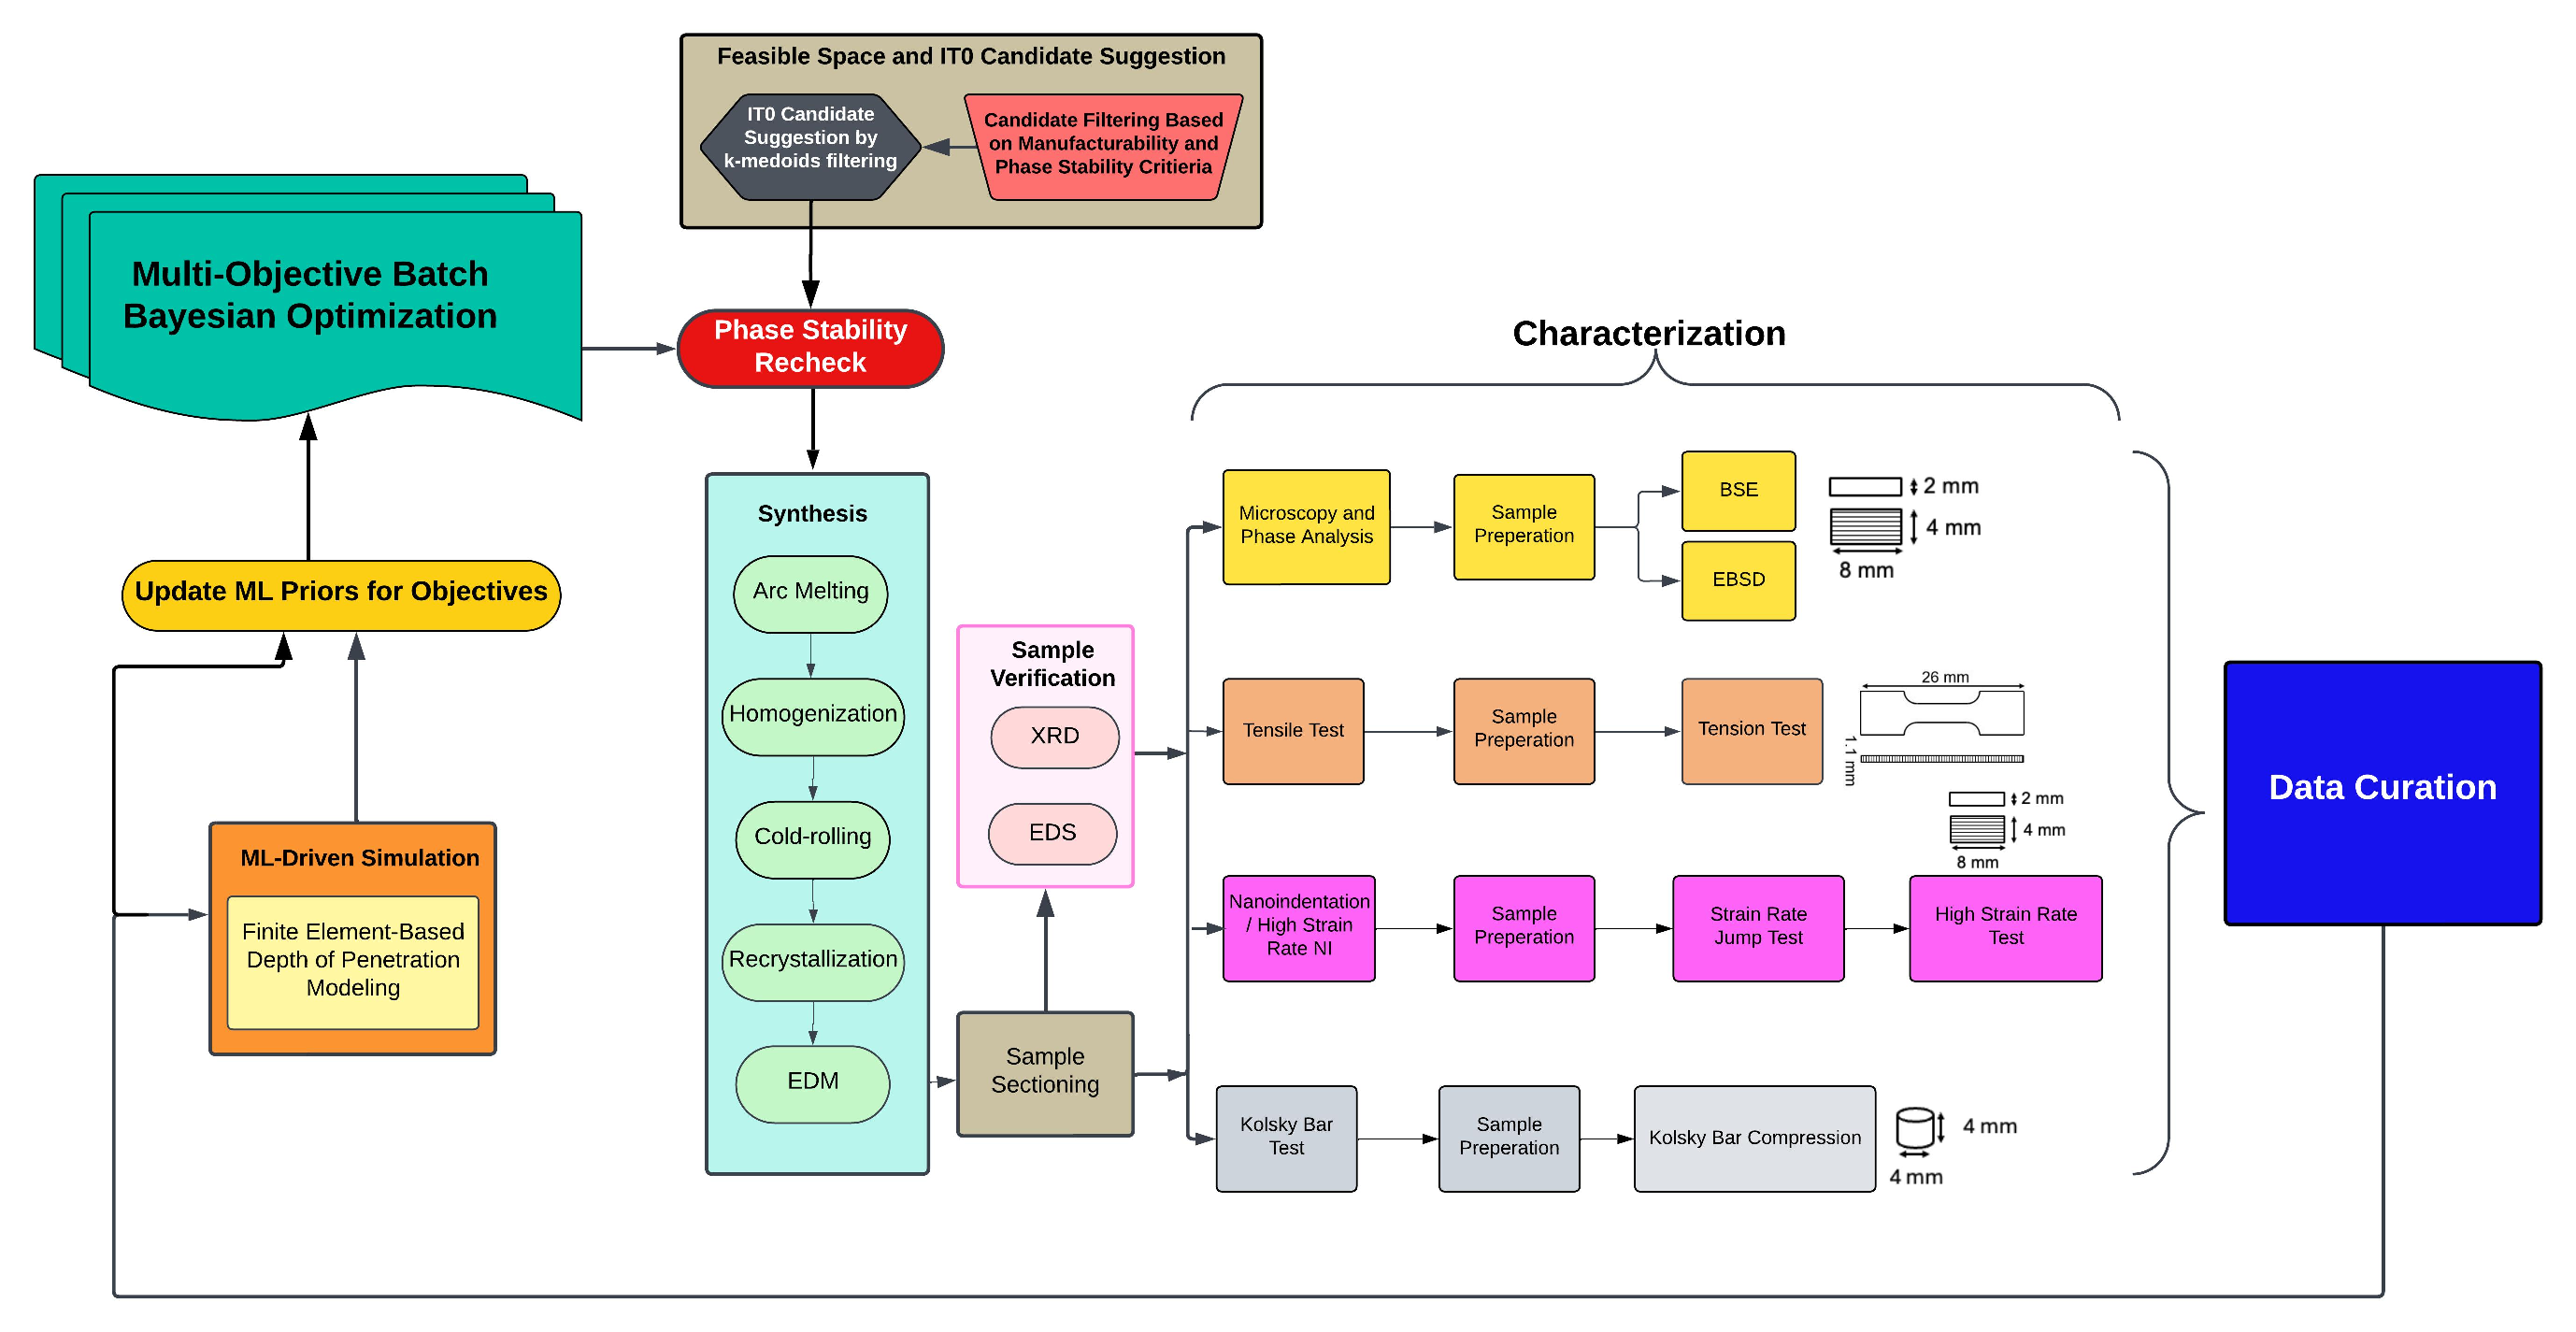
\includegraphics[width=0.95\textwidth]{Sup_figures/fig_si_01_birdshot_workflow.pdf}
    \caption{Integrated BIRDSHOT workflow from candidate suggestion through synthesis, sample preparation, characterization, simulation, and Bayesian optimization for selection of the next batch of candidates.}
    \label{fig:workflow}
\end{figure*}

The mathematical details of the BRAVE computational framework (GP surrogates, informative priors, EHVI acquisition, multi-source fusion, and batch selection) are provided in Appendix~A of the main text.

% GP, Priors, EHVI, Reification, and Batch BO sections moved to main text Appendix A
% (Content removed — now in 05_appendix.tex, Appendix A)


\section{Detailed Sampling and Candidate Selection Strategy for Iteration~0}
\label{sec:supp_sampling_iter0}

\subsection{Overview}

Iteration~0 required selecting a small, manufacturable set of alloys that (i)~lie within a thermodynamically feasible single-phase FCC region, (ii)~span the chemically diverse subspaces of the multi-component system, and (iii)~are compatible with synthesis and characterization constraints. Because the full combinatorial space is extremely large, the selection strategy combined CALPHAD-based thermodynamic screening, manifold learning for exploratory analysis, diversity-aware clustering, and subsystem-balanced down-selection.
\autoref{fig:selection_pipeline} provides a schematic overview of the complete workflow, with each stage annotated by the number of surviving candidates.

\begin{figure}[H]
\centering
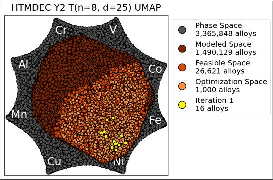
\includegraphics[width=0.9\linewidth]{Sup_figures/fig_si_02_selection_pipeline.pdf}
\caption{Schematic overview of the Iteration~0 candidate selection pipeline, showing the progressive reduction from 3.37~million unconstrained compositions to the final 16-alloy synthesis batch. Each stage is annotated with the number of surviving candidates.}
\label{fig:selection_pipeline}
\end{figure}

\subsection{Compositional Space Enumeration and Subsystem Partitioning}
\label{sec:space_and_subsystems}
 
The design space which is the eight element system Al--V--Cr--Mn--Fe--Co--Ni--Cu, is discretized on a 4~at.\% compositional grid and subject to the simplex constraint $\sum_i x_i = 1$, $x_i \in \{0, 0.04, 0.08, \dots\}$. The number of unique compositions is given by the stars-and-bars formula:
\begin{equation}
T(n, d) = \binom{n + d - 1}{d}, \qquad d = \frac{100}{\Delta},
\label{eq:stars_bars}
\end{equation}
where $n = 8$ and $\Delta = 4$~at.\% yields $d = 25$, giving $T(8, 25) = 3{,}365{,}848$ unique compositions in the unconstrained simplex.
For reference, 2~at.\% and 1~at.\% resolutions yield $264{,}385{,}828$ and $26{,}075{,}972{,}538$ compositions, respectively. \autoref{fig:space_size} illustrates the exponential growth of the combinatorial space with increasing elements and finer discretization.
 
\begin{figure}[!htbp]
\centering
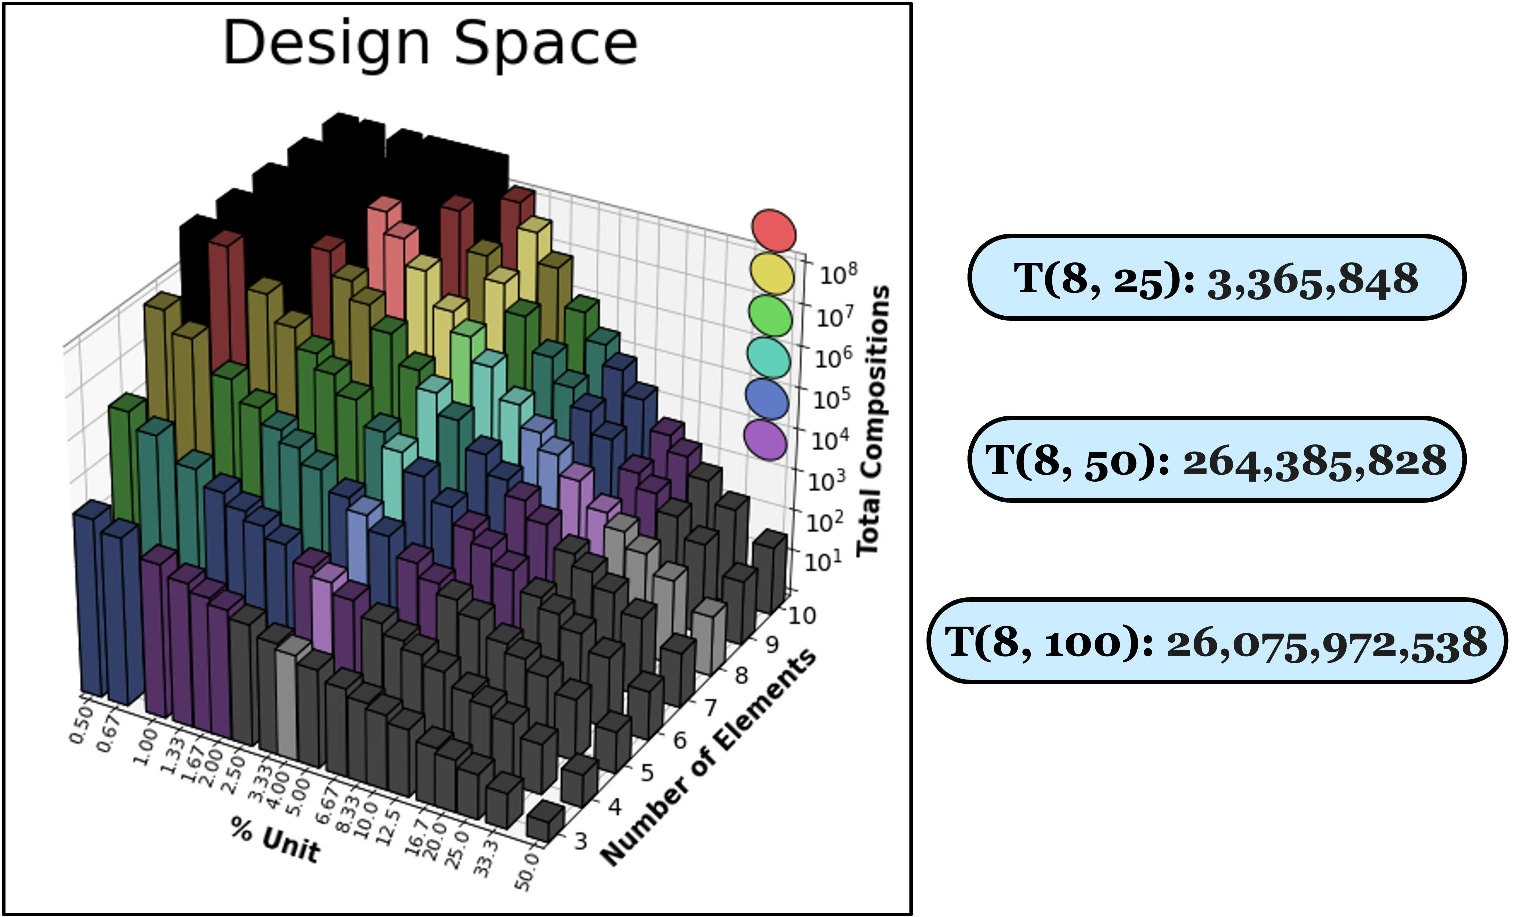
\includegraphics[width=0.9\linewidth]{Sup_figures/fig_si_03_composition_space.pdf}
\caption{Number of unique compositions as a function of system size ($n$~elements) and discretization resolution. The eight-element, 4~at.\% system investigated in this work (red star) contains 3.37~million compositions before applying compositional bounds or phase-stability constraints.}
\label{fig:space_size}
\end{figure}
 
Element specific upper bounds were imposed to ensure manufacturability and avoid extreme chemistries: Al~$\leq$~0.24, V~$\leq$~0.24, Cr~$\leq$~0.50, Mn~$\leq$~0.40, Fe~$\leq$~0.50, Co~$\leq$~0.50, Ni~$\leq$~0.60, and Cu~$\leq$~0.24. Applying these constraints reduced the space to $1{,}504{,}938$ candidate compositions.
 
Each bounded composition was assigned to a chemical subsystem defined by the set of elements present at nonzero atomic fraction on the discretized grid. This partitioning yielded 37 distinct subsystems spanning six- to eight-component alloys (\autoref{tab:subsystems}). The full eight element subsystem (type~1) contains $240{,}000$ compositions after bounding, while seven element subsystems range from $75{,}993$ to $92{,}595$ depending on the excluded element. Six element subsystems show even greater variation, with populations between $15{,}788$ and $29{,}506$. Subsystems of five or fewer elements account for an additional $252{,}629$ compositions. This partitioning was used throughout the pipeline to track chemical diversity and prevent over-sampling of dominant subsystems during candidate selection.
 
\onecolumn
\begin{longtable}{ccccccccccr}
\caption{Chemical subsystem partitioning of the bounded design space. Elements
marked with ** are absent from the subsystem. ``Compositions'' gives the number of grid points in each subsystem after applying element specific upper bounds. Subsystems of size 5 and below are reported as aggregated totals.}
\label{tab:subsystems}\\
\hline
Size & Type & Al & V & Cr & Mn & Fe & Co & Ni & Cu & Compositions \\
\hline
\endfirsthead

\multicolumn{11}{c}{\tablename\ \thetable\ -- \textit{Continued from previous page}} \\
\hline
Size & Type & Al & V & Cr & Mn & Fe & Co & Ni & Cu & Compositions \\
\hline
\endhead

\hline
\multicolumn{11}{r}{\textit{Continued on next page}} \\
\endfoot

\hline
\endlastfoot

8 & 1  & Al & V  & Cr & Mn & Fe & Co & Ni & Cu & 240{,}000 \\
\hline
7 & 2  & Al & V  & Cr & Mn** & Fe & Co & Ni & Cu & 78{,}828 \\
7 & 3  & Al & V  & Cr & Mn & Fe** & Co & Ni & Cu & 76{,}830 \\
7 & 4  & Al & V  & Cr & Mn & Fe & Co & Ni** & Cu & 75{,}993 \\
7 & 5  & Al & V  & Cr** & Mn & Fe & Co & Ni & Cu & 76{,}830 \\
7 & 6  & Al & V** & Cr & Mn & Fe & Co & Ni & Cu & 92{,}595 \\
7 & 7  & Al** & V  & Cr & Mn & Fe & Co & Ni & Cu & 92{,}595 \\
7 & 8  & Al & V  & Cr & Mn & Fe & Co & Ni & Cu** & 92{,}595 \\
7 & 9  & Al & V  & Cr & Mn & Fe & Co** & Ni & Cu & 76{,}830 \\
\hline
6 & 10 & Al & V** & Cr & Mn & Fe & Co & Ni & Cu** & 29{,}506 \\
6 & 11 & Al & V  & Cr** & Mn & Fe & Co & Ni & Cu** & 22{,}584 \\
6 & 12 & Al** & V  & Cr & Mn & Fe & Co & Ni & Cu** & 29{,}506 \\
6 & 13 & Al & V  & Cr & Mn** & Fe & Co & Ni & Cu** & 23{,}694 \\
6 & 14 & Al & V  & Cr & Mn & Fe** & Co & Ni & Cu** & 22{,}584 \\
6 & 15 & Al & V  & Cr & Mn & Fe & Co** & Ni & Cu** & 22{,}584 \\
6 & 16 & Al** & V  & Cr** & Mn & Fe & Co & Ni & Cu & 22{,}584 \\
6 & 17 & Al & V** & Cr & Mn & Fe & Co** & Ni & Cu & 22{,}584 \\
6 & 18 & Al & V  & Cr** & Mn & Fe & Co** & Ni & Cu & 16{,}436 \\
6 & 19 & Al** & V  & Cr & Mn & Fe & Co** & Ni & Cu & 22{,}584 \\
6 & 20 & Al & V  & Cr & Mn & Fe** & Co** & Ni & Cu & 16{,}436 \\
6 & 21 & Al & V  & Cr & Mn** & Fe & Co** & Ni & Cu & 17{,}496 \\
6 & 22 & Al** & V  & Cr & Mn** & Fe & Co & Ni & Cu & 23{,}694 \\
6 & 23 & Al & V** & Cr & Mn** & Fe & Co & Ni & Cu & 23{,}694 \\
6 & 24 & Al** & V** & Cr & Mn & Fe & Co & Ni & Cu & 29{,}506 \\
6 & 25 & Al & V  & Cr & Mn** & Fe** & Co & Ni & Cu & 17{,}496 \\
6 & 26 & Al & V  & Cr** & Mn** & Fe & Co & Ni & Cu & 17{,}496 \\
6 & 27 & Al & V** & Cr & Mn & Fe** & Co & Ni & Cu & 22{,}584 \\
6 & 28 & Al** & V  & Cr & Mn & Fe** & Co & Ni & Cu & 22{,}584 \\
6 & 29 & Al & V  & Cr** & Mn & Fe** & Co & Ni & Cu & 16{,}436 \\
6 & 30 & Al & V** & Cr** & Mn & Fe & Co & Ni & Cu & 22{,}584 \\
6 & 31 & Al & V** & Cr & Mn & Fe & Co & Ni** & Cu & 21{,}930 \\
6 & 32 & Al & V  & Cr & Mn** & Fe & Co & Ni** & Cu & 16{,}848 \\
6 & 33 & Al & V  & Cr** & Mn & Fe & Co & Ni** & Cu & 15{,}788 \\
6 & 34 & Al** & V  & Cr & Mn & Fe & Co & Ni** & Cu & 21{,}930 \\
6 & 35 & Al & V  & Cr & Mn & Fe** & Co & Ni** & Cu & 15{,}788 \\
6 & 36 & Al & V  & Cr & Mn & Fe & Co** & Ni** & Cu & 15{,}788 \\
6 & 37 & Al & V  & Cr & Mn & Fe & Co & Ni** & Cu** & 21{,}930 \\
\hline
5 & all &    &    &    &    &    &    &    &    & 218{,}786 \\
4 & all &    &    &    &    &    &    &    &    & 32{,}285 \\
3 & all &    &    &    &    &    &    &    &    & 1{,}548 \\
2 & all &    &    &    &    &    &    &    &    & 10 \\
\hline
\end{longtable}
\twocolumn

\subsection{CALPHAD Equilibrium Screening}
 
Equilibrium phase fractions were computed at $700\,^{\circ}$C for all $1{,}504{,}938$ bounded compositions using Thermo-Calc~2022.2 with the TCHEA6 database, interfaced through TC-Python. Calculations were parallelized across a high-performance computing cluster and partitioned by chemical subsystem to improve throughput and reduce licensing conflicts. Of the attempted compositions, $1{,}490{,}129$ ($99.02\%$) converged successfully, with peak throughput reaching ${\sim}72{,}000$ equilibrium calculations per core per day and an average of ${\sim}44{,}000$ per core per day. Compositions with predicted FCC phase fraction $\geq 0.99$ were retained as feasible, yielding $27{,}074$ candidates -- $1.54\%$ of the evaluated space (\autoref{fig:fcc_filtering}).
 
\begin{figure}[!htbp]
\centering
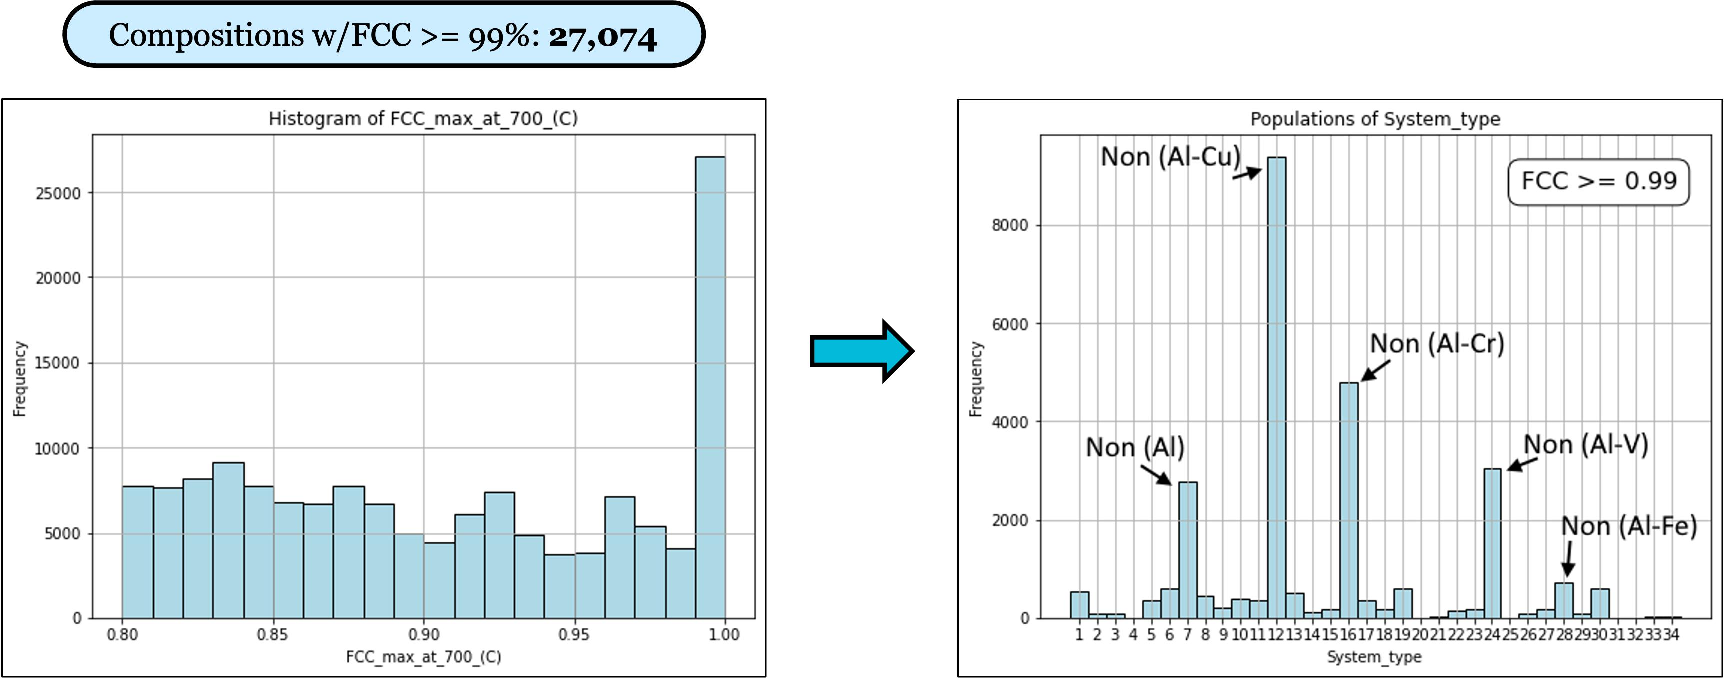
\includegraphics[width=0.9\linewidth]{Sup_figures/fig_si_04_fcc_filtering.pdf}
\caption{Progressive filtering of the design space. Application of the FCC $\geq 0.99$ phase-fraction threshold reduces the modeled space from $1{,}490{,}129$ to $27{,}074$ feasible compositions.}
\label{fig:fcc_filtering}
\end{figure}

\subsection{Local FCC Stability Perturbation Analysis}

To assess how robust CALPHAD-predicted FCC stability is to small local composition changes, we performed a perturbation analysis on candidate alloys that satisfied FCC $\geq 0.99$ (\autoref{fig:perturbation_analysis}. For each candidate composition on the 4~at.\% design grid, we generated nearby compositions by varying each elemental fraction by $\pm 2$~at.\% and recalculated equilibrium phase stability using Thermo-Calc, subject to the composition simplex constraint. This probes whether a composition predicted to be FCC remains FCC under small local composition shifts.

Across 1{,}154{,}207 perturbed compositions evaluated, 903{,}326 retained FCC $\geq 0.99$, corresponding to 78.3\% local phase-stability retention. We therefore interpret a feasibility probability near 0.8 as corresponding to a composition that is locally robust to small perturbations. This provides empirical support for the acquisition threshold $P_\text{feas}(\mathbf{x}) \geq 0.8$ used in the main text.

\begin{figure}[!htbp]
\centering
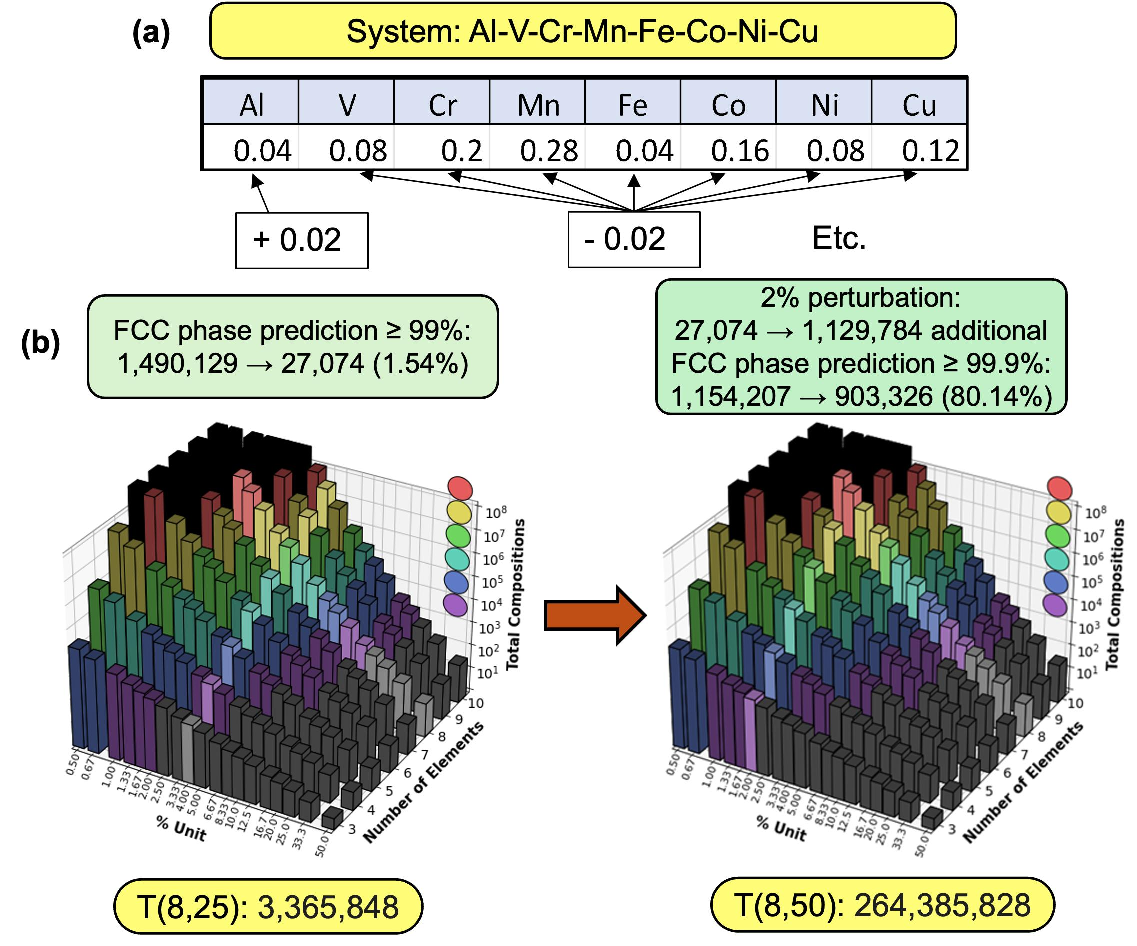
\includegraphics[width=0.9\linewidth]{Sup_figures/fig_si_05_perturbation.pdf}
\caption{Local FCC stability perturbation analysis. (a) Illustration of $\pm$2\,at.\% perturbations in 8D composition space. (b) Distribution of phase-stability outcomes: 78.3\% of perturbed alloys remain fully FCC (FCC $\geq 0.99$), while the remainder show secondary phases such as BCC or SIGMA.}
\label{fig:perturbation_analysis}
\end{figure}

\subsection{Observations from FCC Feasibility Screening}
 
The FCC screening results show several structural features of the feasible design space. Nickel is essential for FCC stability in this system: all subsystems lacking nickel, including types~4, 31--37, and all five-element and smaller subsystems without nickel returned zero viable candidates at the $\geq 0.99$ FCC threshold. The maximum FCC phase fraction achieved by any nickel-free composition remained below 0.90 (type~4), with some subsystems not exceeding 0.87--0.88 (types~31, 32). In contrast, cobalt-free subsystems (types~9, 15, 17--21) retained thousands of feasible compositions.
 
Effective solubility limits imposed by the FCC stability constraint differ markedly from the imposed compositional bounds. Copper, although bounded at 0.24, is effectively confined to much lower concentrations in FCC feasible compositions, reflecting limited solid solubility in the FCC matrix. Chromium is similarly constrained, with feasible compositions not exceeding ${\sim}28$~at.\% despite a bound of 0.50. Nickel, by contrast, occupies the highest atomic fractions among the feasible candidates, consistent with its role as the primary FCC stabilizer.
 
The strong population imbalance across subsystems (\autoref{fig:subsystem_counts}) has direct implications for sampling: naive random selection from the $27{,}074$ feasible compositions would over-represent high-population subsystems and miss chemically distinct but sparsely populated regions. Subsystems with fewer than 100 FCC-feasible candidates were excluded, retaining $26{,}621$ compositions across the feasible subsystems for subsequent clustering.
 
\begin{figure}[!htbp]
\centering
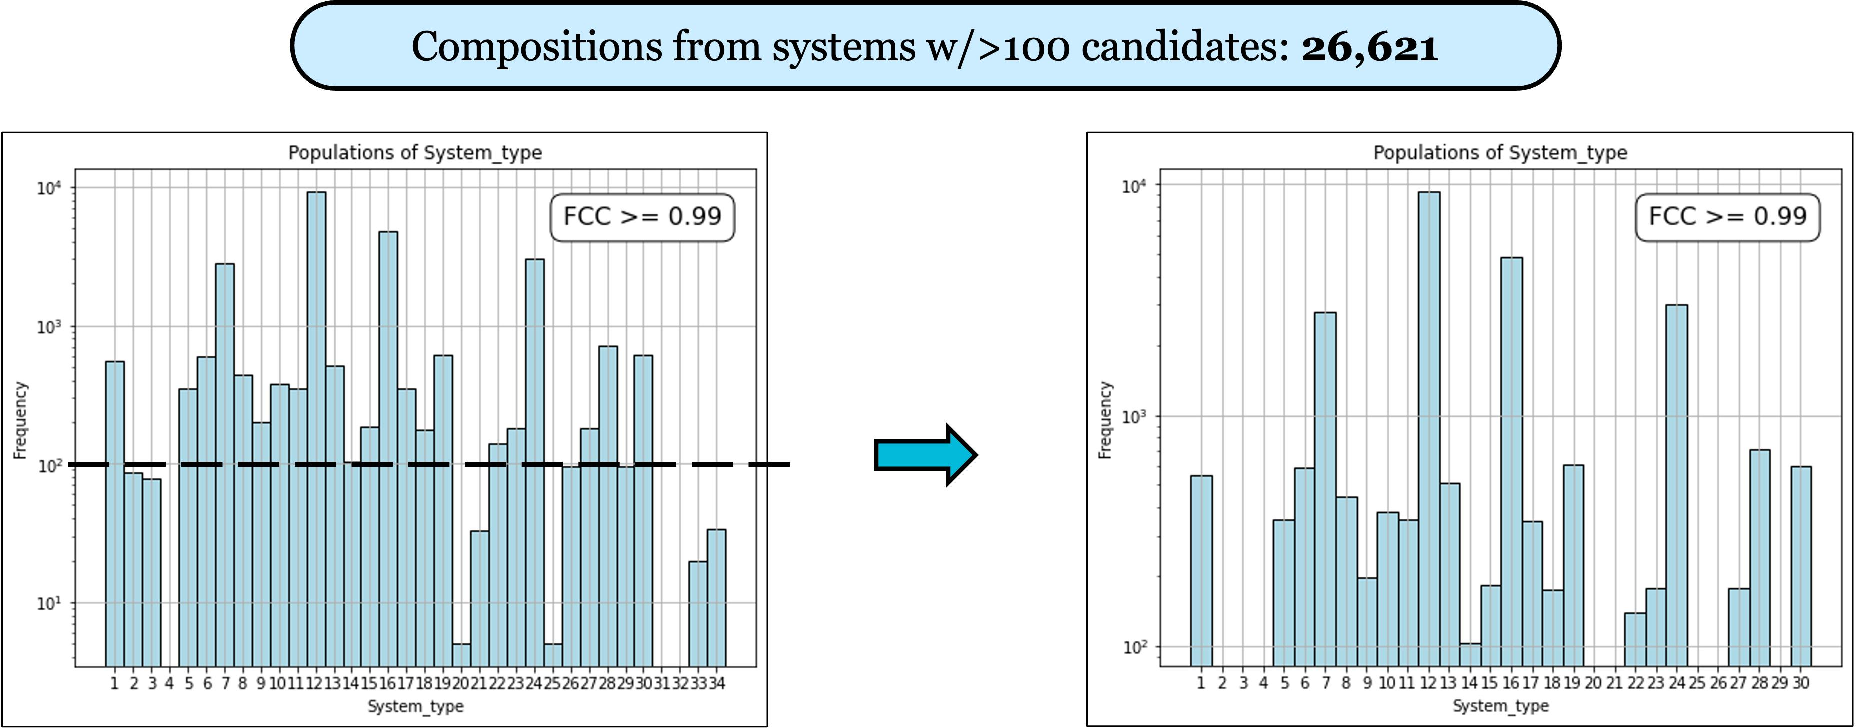
\includegraphics[width=0.9\linewidth]{Sup_figures/fig_si_06_subsystem_counts.pdf}
\caption{Number of FCC-feasible compositions per chemical subsystem, showing strong population imbalance. Subsystems with fewer than 100 candidates were excluded from subsequent sampling, retaining $26{,}621$ compositions.}
\label{fig:subsystem_counts}
\end{figure}
 
\subsection{Diversity Sampling via $k$-Medoids Clustering}
 
To construct a representative and computationally manageable subset, $k$-medoids clustering was applied to the atomic-fraction vectors of the $26{,}621$ viable compositions using Euclidean distance, with $k = 1{,}000$. Because medoids are actual data points, all selected representatives are physically realizable compositions. The 1{,}000 medoids span both high density core regions and peripheral areas of the feasible space. Standard initialization using only atomic fractions as dimensions tends to favor high population subsystems; explicit subsystem aware down selection (described below) was therefore required to ensure chemical diversity in the final batch.
 
\subsection{Down Selection to the Iteration~0 Batch}
 
The final Iteration~0 (BBA) batch consisted of 16 alloys (\autoref{fig:BBA}, constrained by experimental throughput. Down selection from the 1{,}000 medoids used a quota-based diversity algorithm to ensure coverage across chemical subsystems.
Each subsystem $i$ was assigned a quota
\[
q_i = \max\!\left(1, \;\mathrm{round}\!\left(16 \cdot \frac{n_i}{\textstyle\sum_j n_j}\right)\right),
\]
where $n_i$ is the number of feasible candidates in subsystem $i$, with greedy correction to enforce $\sum_i q_i = 16$. Within each subsystem, medoids were ranked by a combined criterion balancing proximity to the subsystem centroid (representativeness) and distance from the global centroid (chemical diversity). A final greedy refinement step maximized the minimum pairwise distance among the 16 selected candidates.

\begin{figure*}[t]
    \centering
    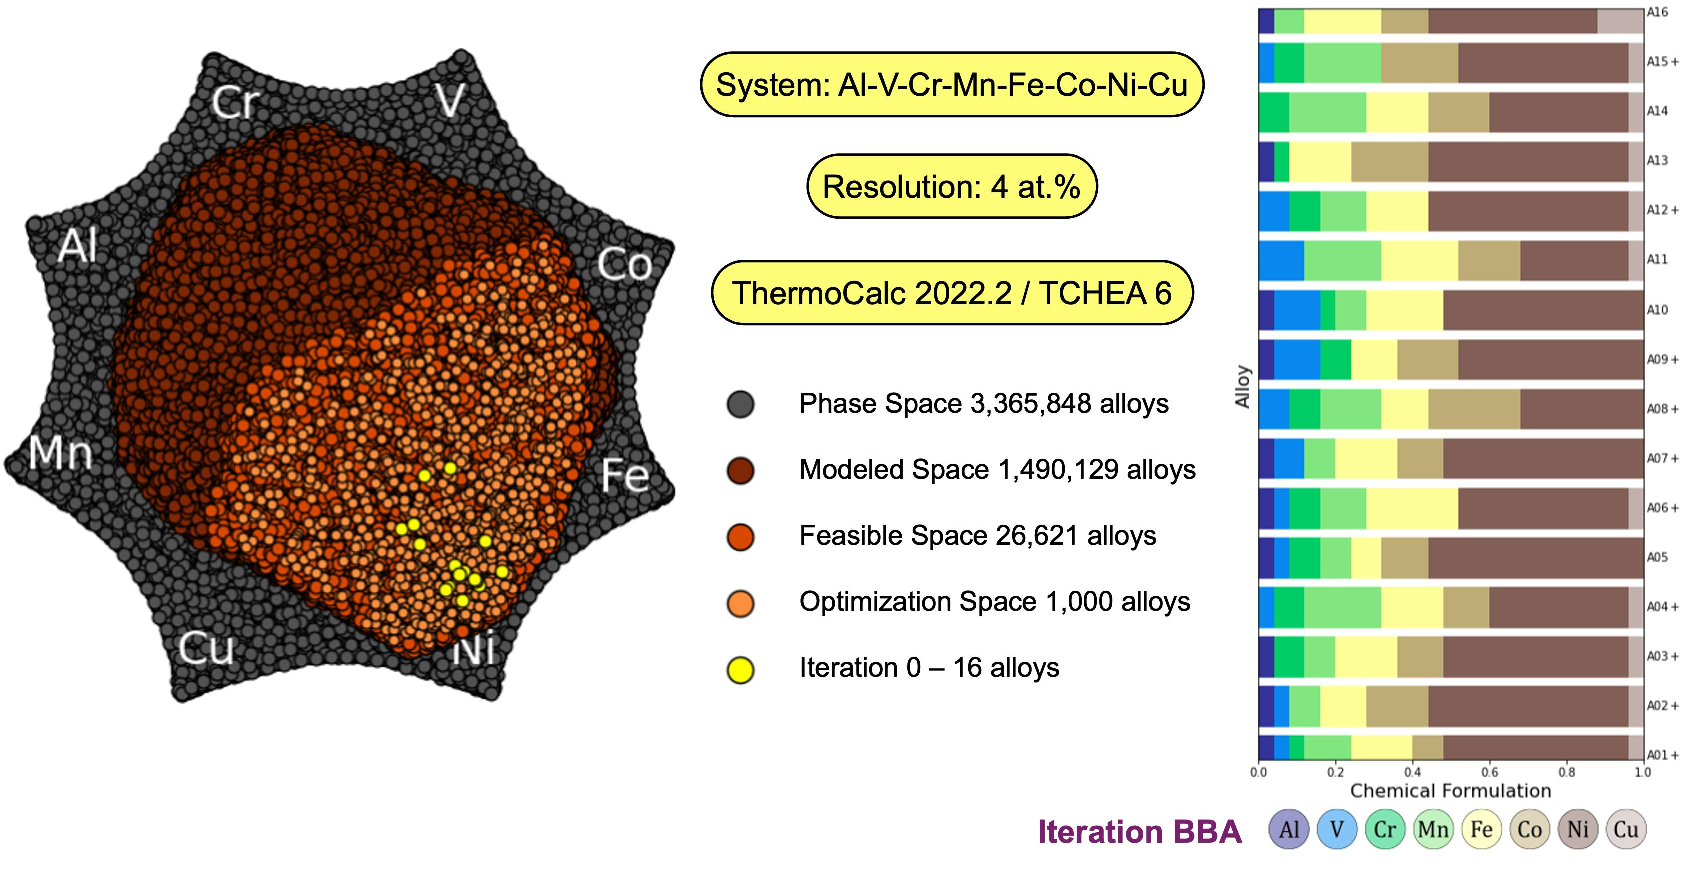
\includegraphics[width=0.8\textwidth]{Sup_figures/fig_si_07_bba_suggestions.pdf}
    \caption{Candidate alloy suggestions for Iteration 0 (BBA), selected by diversity-aware $k$-medoids sampling across 37 chemical subsystems.}
    \label{fig:BBA}
\end{figure*}


\newpage
\section{High-Throughput Sample Preparation, Characterization Automation, and Data Management}
\label{s1_htp_workflow}

\subsection{Sample Preparation Workflow Evolution}

Microstructural characterization and nanoindentation samples were initially prepared by mechanical polishing using a Buehler AutoMet 250 autopolisher with diamond suspensions down to 1~$\mu$m. For electron backscatter diffraction (EBSD) analysis, the surfaces were subsequently polished to a mirror finish using a Buehler VibroMet 2 vibratory polisher for 12~h in a 0.04~$\mu$m colloidal silica suspension.

In iterations BBA and BBB, samples were individually mounted using graphite mounting powder. Although effective, this method was labor-intensive and caused misalignment during indentation testing in a few cases. In addition, it limited batch sizes to eight samples, thereby reducing throughput. To improve efficiency and sample quality, a new preparation technique was developed in iteration BBC. This revised protocol used large aluminum polishing platens that allowed simultaneous processing of 16 or more samples. Samples were fixed to these platens using crystalbond adhesive, ensuring uniform mounting height and eliminating misalignment issues that had previously impacted mechanical characterization.

To prevent sample mix-ups during high-throughput processing, a laser marking system was introduced. Each sample is lightly marked on its reverse side with a unique identifier indicating the iteration and sample number. Although this step adds to the workflow, it has been optimized for rapid batch processing and ensures reliable traceability throughout testing.

Future plans aim to further increase efficiency by adapting techniques that enable mounting of eight samples per aluminum puck. This adjustment will allow up to 48 samples to be ground and polished concurrently, while maintaining the precise alignment required for subsequent mechanical testing. Overall, these improvements are projected to result in a sixfold increase in sample preparation throughput compared to the initial methods.

\subsection{Nanoindentation and High Strain Rate Nanoindentation Automation}

Custom Python and ImageJ scripts were implemented to automate image acquisition and projected contact area analysis for nanoindentation, addressing one of the primary challenges in establishing an automated system for measuring contact area. Ensuring consistent reliability across different materials and strain rates was a critical hurdle that was overcome through iterative refinements. These improvements enabled direct comparisons between nanoindentation data and results from high strain rate methods, such as the split Hopkinson pressure bar. The strain rate sensitivities obtained from these different techniques were found to be in close agreement, typically within one standard deviation.

Integrating the high strain rate nanoindentation system into the workflow presented additional technical challenges. The instrument outputs data in encrypted binary files, which required development of Python scripts for reliable data extraction. Further automation scripts were developed to handle complex data analysis tasks, reducing processing time. Nanoindentation data was cross-validated with tensile and Hopkinson bar test results to identify correlations in rate sensitivity across the three measurement techniques. The rate sensitivities from all methods were found to be within one standard deviation of each other.

\subsection{Data Management Architecture}

Data management in the prior BIRDSHOT study was organized around a \textbf{sample-centric framework}, designed to meet the distinct requirements of the VAM and DED synthesis workflows \cite{mulukutla2024illustrating}. This approach enabled end-to-end traceability from synthesis through characterization and analysis, supporting distributed collaboration and ensuring data integrity via natural version control. However, the path-dependent folder navigation imposed significant challenges for new users and complicated retrieval of specific results even for existing users. This experience motivated the adoption of a more discoverable, database-driven framework in subsequent studies.

In the current BIRDSHOT study, we implemented a \textbf{method-centric data architecture}, as shown in \autoref{fig:method_structure_si}, designed to maximize traceability, scalability, and efficiency while reducing redundancy. In this system, sample identifiers remain linked to synthesis origin, but folder organization treats design, processing and characterization methods as first-class entities beneath synthesis-level groupings. Sample folders use short, descriptive labels (e.g., \texttt{SEM}, \texttt{Tensile}, \texttt{NI}) to enable rapid identification, and measurement identifiers follow a hierarchical and extensible convention \texttt{<SampleID>\_\allowbreak<Synthesis>\_\allowbreak<Technique>[\_\allowbreak<Subsample>][\_\allowbreak...]}. Metadata associated with each method, such as \texttt{sem-details.json} or \texttt{tensile-details.json}, is stored in structured JSON files within the corresponding method folders, allowing automated parsing, integration with downstream analysis pipelines, and programmatic traversal. For high-throughput synthesis, folders labeled by production batch capture shared processing metadata to minimize duplication while maintaining logical clarity and supporting future extensibility for new characterization techniques or processing steps.

\begin{figure}[htbp]
    \centering
    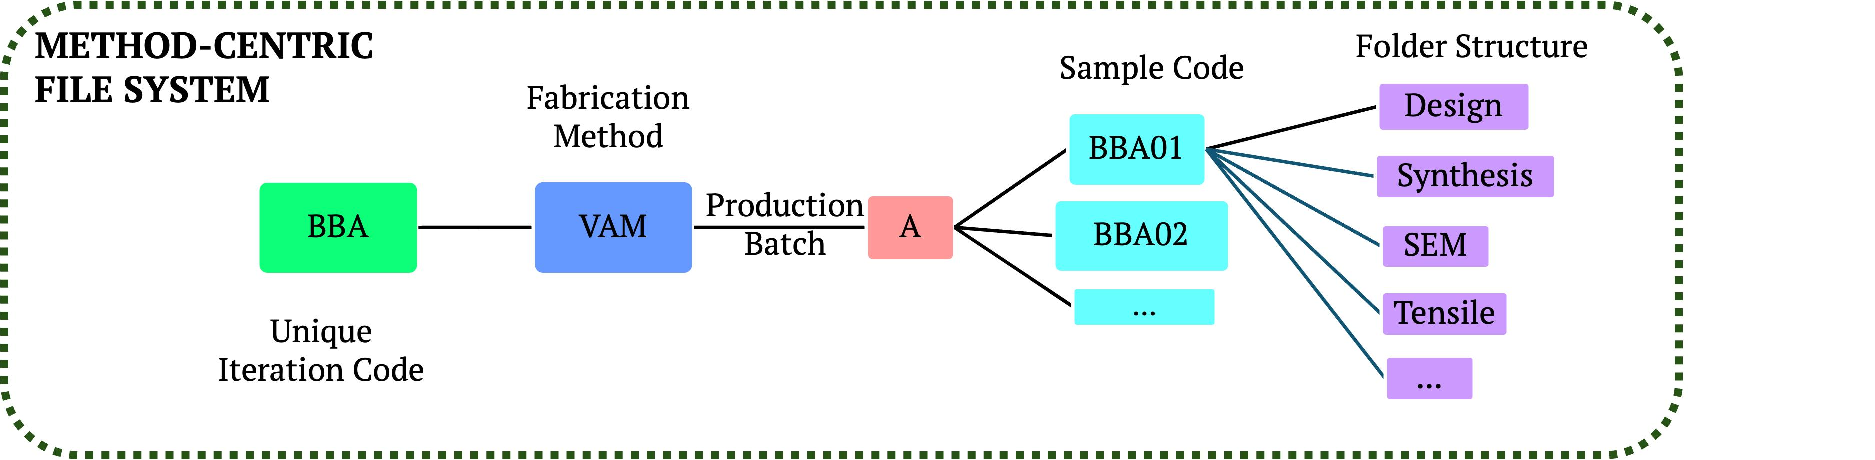
\includegraphics[width=0.9\columnwidth]{Sup_figures/fig_si_08_file_structure.pdf}
    \caption{Folder structure illustrating synthesis-level grouping and method-focused organization.}
    \label{fig:method_structure_si}
\end{figure}

\subsection{IGSN Sample Registration}

Each candidate alloy in this study is assigned an International Generic Sample Number (IGSN), a globally unique, resolvable identifier for physical samples, thereby linking the physical specimens, their metadata, and downstream analytical results in a persistent, cross-platform framework. IGSNs are issued and managed under the IGSN--DataCite partnership, ensuring sustainability and interoperability across research data systems \cite{datacite-igsn-ids}.

By design, IGSN identifiers behave like DOIs: they are registered in a dedicated IGSN catalog within the DataCite system and resolved using standard DOI infrastructure, but are distinguished semantically as ``physical object'' identifiers. The metadata for each IGSN follows the DataCite Metadata Schema, including mandatory fields such as identifier, creator, title, publisher, publication year, and resource type, along with recommended fields like related identifier, contributors, dates, descriptions, and geolocation when applicable \cite{igsn-metadata-schema}. In particular, our sample hierarchy is reflected in the related Identifier fields so that parent--child relationships (like subsamples) are explicitly recorded in the IGSN metadata. Because IGSNs are globally registered and resolvable, they support FAIR principles---especially findability and interoperability---by enabling external users (or data infrastructures) to unambiguously reference and access sample information, even beyond our internal data ecosystem.


\section{IGSN Metadata and Compositions for All Alloys}
\label{s1_igsn_compositions}

All alloys synthesized in this study are registered with International Generic Sample Numbers (IGSNs) through the DataCite system. Each IGSN is resolvable via the IGSN ID service (\url{https://support.datacite.org/docs/igsn-ids}). \autoref{table_igsn_bba}, \autoref{table_igsn_bbb}, and \autoref{table_igsn_bbc} list the alloy identifier, target composition (at.\%), and IGSN for every alloy across the three design iterations.

\cleardoublepage
\onecolumn
\subsection{\texorpdfstring{\textbf{Supplementary \autoref{table_igsn_bba}} \texorpdfstring{$\mid\;$}{Lg}Iteration 0 (BBA) alloys}{Supplementary Table -- Iteration 0 (BBA) alloys}}
\label{s1_igsn_bba}
\vspace{-1em}

\begin{table}[H]
\caption{}
\label{table_igsn_bba}
\begin{tblr}{
    hlines,
    hline{3,22} = {2pt},
    rowsep=1pt,
    colspec = {
        |X[1.2, c]
        |[2pt]X[0.7, c]|X[0.7, c]|X[0.7, c]|X[0.7, c]|X[0.7, c]|X[0.7, c]|X[0.7, c]|X[0.7, c]
        |[2pt]X[2.0, c]|
        },
    colsep=0pt,
    }
    \SetCell[r=2,c=1]{c}\textbf{\makecell{Alloy\\Name}}
    & \SetCell[c=8]{c} \textbf{Target Atomic \%}
    &&&&&&&
    & \SetCell[r=2,c=1]{c}\textbf{IGSN} \\
    & Al & Co & Cr & Cu & Fe & Mn & Ni & V & \\
    BBA01 & 4 & 8 & 4 & 4 & 16 & 12 & 48 & 4 & TMAMAK00097 \\
    BBA02 & 4 & 16 & \SetCell{gray!20}0 & 4 & 12 & 8 & 52 & 4 & TMAMAK00098 \\
    BBA03 & 4 & 12 & 8 & 4 & 16 & 8 & 48 & \SetCell{gray!20}0 & TMAMAK00099 \\
    BBA04 & \SetCell{gray!20}0 & 12 & 8 & 4 & 16 & 20 & 36 & 4 & TMAMAK00100 \\
    BBA05 & 4 & 12 & 8 & \SetCell{gray!20}0 & 8 & 8 & 56 & 4 & TMAMAK00101 \\
    BBA06 & 4 & \SetCell{gray!20}0 & 8 & 4 & 24 & 12 & 44 & 4 & TMAMAK00102 \\
    BBA07 & 4 & 12 & \SetCell{gray!20}0 & \SetCell{gray!20}0 & 16 & 8 & 52 & 8 & TMAMAK00103 \\
    BBA08 & \SetCell{gray!20}0 & 24 & 8 & \SetCell{gray!20}0 & 12 & 16 & 32 & 8 & TMAMAK00104 \\
    BBA09 & 4 & 16 & 8 & \SetCell{gray!20}0 & 12 & \SetCell{gray!20}0 & 48 & 12 & TMAMAK00105 \\
    BBA10 & 4 & \SetCell{gray!20}0 & 4 & \SetCell{gray!20}0 & 20 & 8 & 52 & 12 & TMAMAK00106 \\
    BBA11 & \SetCell{gray!20}0 & 16 & \SetCell{gray!20}0 & 4 & 20 & 20 & 28 & 12 & TMAMAK00107 \\
    BBA12 & \SetCell{gray!20}0 & \SetCell{gray!20}0 & 8 & 4 & 16 & 12 & 52 & 8 & TMAMAK00108 \\
    BBA13 & 4 & 20 & 4 & 4 & 16 & \SetCell{gray!20}0 & 52 & \SetCell{gray!20}0 & TMAMAK00109 \\
    BBA14 & \SetCell{gray!20}0 & 16 & 8 & 4 & 16 & 20 & 36 & \SetCell{gray!20}0 & TMAMAK00110 \\
    BBA15 & \SetCell{gray!20}0 & 20 & 8 & 4 & \SetCell{gray!20}0 & 20 & 44 & 4 & TMAMAK00111 \\
    BBA16 & 4 & 12 & \SetCell{gray!20}0 & 12 & 20 & 8 & 44 & \SetCell{gray!20}0 & TMAMAK00112 \\
\end{tblr}
\end{table}


\subsection{\texorpdfstring{\textbf{Supplementary \autoref{table_igsn_bbb}} \texorpdfstring{$\mid\;$}{Lg}Iteration 1 (BBB) alloys}{Supplementary Table -- Iteration 1 (BBB) alloys}}
\label{s1_igsn_bbb}
\vspace{-1em}

\begin{table}[H]
\caption{}
\label{table_igsn_bbb}
\begin{tblr}{
    hlines,
    hline{3,19} = {2pt},
    rowsep=1pt,
    colspec = {
        |X[1.2, c]
        |[2pt]X[0.7, c]|X[0.7, c]|X[0.7, c]|X[0.7, c]|X[0.7, c]|X[0.7, c]|X[0.7, c]|X[0.7, c]
        |[2pt]X[2.0, c]|
        },
    colsep=0pt,
    }
    \SetCell[r=2,c=1]{c}\textbf{\makecell{Alloy\\Name}}
    & \SetCell[c=8]{c} \textbf{Target Atomic \%}
    &&&&&&&
    & \SetCell[r=2,c=1]{c}\textbf{IGSN} \\
    & Al & Co & Cr & Cu & Fe & Mn & Ni & V & \\
    BBB01 & \SetCell{gray!20}0 & 24 & 4 & \SetCell{gray!20}0 & 8 & 4 & 36 & 24 & TMAMAK00113 \\
    BBB02 & 4 & 32 & 8 & 4 & 4 & 20 & 24 & 4 & TMAMAK00114 \\
    BBB03 & 4 & \SetCell{gray!20}0 & 12 & 4 & 4 & 16 & 52 & 8 & TMAMAK00115 \\
    BBB04 & 4 & 12 & 4 & \SetCell{gray!20}0 & 28 & \SetCell{gray!20}0 & 40 & 12 & TMAMAK00116 \\
    BBB05 & \SetCell{gray!20}0 & 44 & 12 & \SetCell{gray!20}0 & 4 & 4 & 12 & 24 & TMAMAK00117 \\
    BBB06 & \SetCell{gray!20}0 & 16 & 20 & \SetCell{gray!20}0 & 4 & 4 & 36 & 20 & TMAMAK00118 \\
    BBB07 & 4 & 40 & \SetCell{gray!20}0 & \SetCell{gray!20}0 & 12 & 4 & 36 & 4 & TMAMAK00119 \\
    BBB08 & 4 & 8 & 12 & 4 & 4 & 24 & 40 & 4 & TMAMAK00120 \\
    BBB09 & \SetCell{gray!20}0 & 4 & 8 & \SetCell{gray!20}0 & 4 & 28 & 40 & 16 & TMAMAK00121 \\
    BBB10 & 4 & \SetCell{gray!20}0 & 4 & 4 & 8 & 16 & 52 & 12 & TMAMAK00122 \\
    BBB11 & \SetCell{gray!20}0 & 24 & 4 & \SetCell{gray!20}0 & 4 & 32 & 20 & 16 & TMAMAK00123 \\
    BBB12 & \SetCell{gray!20}0 & 20 & 4 & \SetCell{gray!20}0 & 4 & 4 & 48 & 20 & TMAMAK00124 \\
    BBB13 & \SetCell{gray!20}0 & 40 & 4 & \SetCell{gray!20}0 & 28 & 4 & 4 & 20 & TMAMAK00125 \\
    BBB14 & 4 & \SetCell{gray!20}0 & 12 & 16 & 4 & 12 & 52 & \SetCell{gray!20}0 & TMAMAK00126 \\
    BBB15 & 4 & \SetCell{gray!20}0 & 8 & 24 & 4 & 16 & 44 & \SetCell{gray!20}0 & TMAMAK00127 \\
    BBB16 & 4 & 36 & \SetCell{gray!20}0 & \SetCell{gray!20}0 & 4 & 4 & 40 & 12 & TMAMAK00128 \\
\end{tblr}
\end{table}


\subsection{\texorpdfstring{\textbf{Supplementary \autoref{table_igsn_bbc}} \texorpdfstring{$\mid\;$}{Lg}Iteration 2 (BBC) alloys}{Supplementary Table -- Iteration 2 (BBC) alloys}}
\label{s1_igsn_bbc}
\vspace{-1em}

\begin{table}[H]
\caption{}
\label{table_igsn_bbc}
\begin{tblr}{
    hlines,
    hline{3,19} = {2pt},
    rowsep=1pt,
    colspec = {
        |X[1.2, c]
        |[2pt]X[0.7, c]|X[0.7, c]|X[0.7, c]|X[0.7, c]|X[0.7, c]|X[0.7, c]|X[0.7, c]|X[0.7, c]
        |[2pt]X[2.0, c]|
        },
    colsep=0pt,
    }
    \SetCell[r=2,c=1]{c}\textbf{\makecell{Alloy\\Name}}
    & \SetCell[c=8]{c} \textbf{Target Atomic \%}
    &&&&&&&
    & \SetCell[r=2,c=1]{c}\textbf{IGSN} \\
    & Al & Co & Cr & Cu & Fe & Mn & Ni & V & \\
    BBC01 & 4 & 12 & 4 & 4 & 20 & 16 & 32 & 8 & TMAMAK00129 \\
    BBC02 & 4 & 8 & \SetCell{gray!20}0 & \SetCell{gray!20}0 & 4 & 8 & 52 & 24 & TMAMAK00130 \\
    BBC03 & 4 & 4 & 12 & \SetCell{gray!20}0 & \SetCell{gray!20}0 & 4 & 52 & 24 & TMAMAK00131 \\
    BBC04 & 4 & \SetCell{gray!20}0 & 4 & \SetCell{gray!20}0 & 4 & 4 & 60 & 24 & TMAMAK00132 \\
    BBC05 & \SetCell{gray!20}0 & 24 & 8 & \SetCell{gray!20}0 & 16 & 40 & 4 & 8 & TMAMAK00133 \\
    BBC06 & 4 & 28 & 4 & \SetCell{gray!20}0 & 4 & 4 & 44 & 12 & TMAMAK00134 \\
    BBC07 & 4 & 32 & 4 & \SetCell{gray!20}0 & \SetCell{gray!20}0 & 4 & 44 & 12 & TMAMAK00135 \\
    BBC08 & \SetCell{gray!20}0 & 8 & \SetCell{gray!20}0 & 4 & 4 & 28 & 36 & 20 & TMAMAK00136 \\
    BBC09 & \SetCell{gray!20}0 & 36 & 4 & \SetCell{gray!20}0 & 16 & 16 & 8 & 20 & TMAMAK00137 \\
    BBC10 & 4 & 4 & 16 & \SetCell{gray!20}0 & 8 & \SetCell{gray!20}0 & 52 & 16 & TMAMAK00138 \\
    BBC11 & 4 & 12 & 4 & 4 & 12 & 16 & 36 & 12 & TMAMAK00139 \\
    BBC12 & 4 & 4 & 4 & 8 & 28 & 16 & 32 & 4 & TMAMAK00140 \\
    BBC13 & 4 & 28 & \SetCell{gray!20}0 & 20 & 4 & 8 & 36 & \SetCell{gray!20}0 & TMAMAK00141 \\
    BBC14 & \SetCell{gray!20}0 & 12 & 4 & \SetCell{gray!20}0 & 4 & 16 & 40 & 24 & TMAMAK00142 \\
    BBC15 & 4 & 16 & \SetCell{gray!20}0 & 20 & 4 & 12 & 44 & \SetCell{gray!20}0 & TMAMAK00143 \\
    BBC16 & 4 & 28 & 4 & \SetCell{gray!20}0 & 8 & \SetCell{gray!20}0 & 40 & 16 & TMAMAK00144 \\
\end{tblr}
\end{table}
\twocolumn


\section{TCHEA6 to TCHEA7 Database Update: Ternary Subsystem Coverage}
\label{s1_tchea7_update}

During this study, Thermo-Calc released the updated TCHEA7 database with refined phase stability predictions across more than 100 ternary and higher order systems. To assess the impact on the Al--V--Cr--Mn--Fe--Co--Ni--Cu design space, all 56 ternary subsystems were evaluated for assessment availability in both TCHEA6 and TCHEA7, along with any newly predicted secondary phases (sigma, BCC, FCC, HCP). \autoref{tab:tchea7_update} summarizes the results. A ``Yes'' in only the TCHEA7 column indicates a newly added assessment; ``Yes'' in both columns indicates an assessment that was already available in TCHEA6 and carried over; blank or ``No'' entries indicate no assessment is available.

Key changes from TCHEA6 to TCHEA7 relevant to this campaign include the addition of sigma phase predictions in several subsystems (e.g., V--Cr--Fe, V--Cr--Co, V--Fe--Co), new BCC predictions (V--Co--Ni, Fe--Ni--Cu, Co--Ni--Cu), and expanded HCP phase assessments in multiple subsystems (Al--Cr--Ni, Al--Mn--Fe, Al--Co--Ni, Al--Ni--Cu, V--Fe--Ni, Cr--Fe--Ni, Mn--Fe--Cu, Mn--Ni--Cu, Fe--Co--Cu, Fe--Ni--Cu, Co--Ni--Cu). Of particular relevance to this campaign, the V--Cr--Fe and V--Fe--Ni subsystems (highlighted in \autoref{tab:tchea7_update}) received updated assessments that introduced sigma, FCC, and HCP phase predictions not present in TCHEA6. Several alloys containing these ternary combinations showed secondary phases experimentally, consistent with the refined TCHEA7 predictions. These updates motivated the rescreening of the full feasible space using TCHEA7 with the additional constraint of FCC~$\geq 0.99$ at $950\,^{\circ}$C, as described in the main text.

\onecolumn
\small
\begin{longtable}{lcccccc}
\caption{Ternary subsystem assessment availability in TCHEA6 and TCHEA7 for the Al--V--Cr--Mn--Fe--Co--Ni--Cu system. ``Yes'' in both columns indicates the assessment was available in TCHEA6 and carried over; ``Yes'' in only the TCHEA7 column indicates a newly added assessment; blank or ``No'' indicates no assessment is available. Additional columns indicate whether sigma, BCC, FCC, or HCP phases are newly predicted in TCHEA7 for that subsystem. Bold rows indicate subsystems where experimentally observed secondary phases align with the updated TCHEA7 predictions.}
\label{tab:tchea7_update} \\
 
\hline
\textbf{Subsystem} & \textbf{TCHEA6} & \textbf{TCHEA7} & \textbf{SIGMA} & \textbf{BCC} & \textbf{FCC} & \textbf{HCP} \\
\hline
\endfirsthead
 
\hline
\textbf{Subsystem} & \textbf{TCHEA6} & \textbf{TCHEA7} & \textbf{SIGMA} & \textbf{BCC} & \textbf{FCC} & \textbf{HCP} \\
\hline
\endhead
 
\hline
\multicolumn{7}{r}{\textit{Continued on next page}} \\
\endfoot
 
\hline
\endlastfoot
 
\multicolumn{7}{l}{\textit{Al--V--X}} \\
Al--V--Cr   & Yes & Yes &  SIGMA &     &     &     \\
Al--V--Mn   &     & No  &        &     &     &     \\
Al--V--Fe   & No  & No  &  SIGMA &     &     &     \\
Al--V--Co   & No  & No  &  SIGMA &     &     &     \\
Al--V--Ni   & Yes & Yes &  SIGMA &     &     &     \\
Al--V--Cu   &     & No  &        &     &     &     \\
\hline
\multicolumn{7}{l}{\textit{Al--Cr--X}} \\
Al--Cr--Mn  &     & No  &        &     &     &     \\
Al--Cr--Fe  & Yes & Yes &        &     &     &     \\
Al--Cr--Co  & Yes & Yes &  SIGMA &     &     &     \\
Al--Cr--Ni  & Yes & Yes &  SIGMA &     &     & HCP \\
Al--Cr--Cu  &     & No  &        &     &     &     \\
\hline
\multicolumn{7}{l}{\textit{Al--Mn--X}} \\
Al--Mn--Fe  &     & Yes &        &     &     & HCP \\
Al--Mn--Co  &     & No  &        &     &     &     \\
Al--Mn--Ni  &     & Yes &        &     &     &     \\
Al--Mn--Cu  &     & Yes &        &     &     &     \\
\hline
\multicolumn{7}{l}{\textit{Al--Fe--X}} \\
Al--Fe--Co  & No  & No  &        &     &     &     \\
Al--Fe--Ni  & Yes & Yes &  SIGMA &     &     & HCP \\
Al--Fe--Cu  &     & Yes &        &     &     &     \\
\hline
\multicolumn{7}{l}{\textit{Al--Co--X}} \\
Al--Co--Ni  & Yes & Yes &        &     &     & HCP \\
Al--Co--Cu  &     & No  &        &     &     &     \\
\hline
\multicolumn{7}{l}{\textit{Al--Ni--X}} \\
Al--Ni--Cu  &     & Yes &        &     &     & HCP \\
\hline
\multicolumn{7}{l}{\textit{V--Cr--X}} \\
V--Cr--Mn   &     & No  &        &     &     &     \\
\textbf{V--Cr--Fe}   & \textbf{Yes} & \textbf{Yes} & \textbf{SIGMA} &     & \textbf{FCC} & \textbf{HCP} \\
V--Cr--Co   & Yes & Yes &  SIGMA &     &     &     \\
V--Cr--Ni   & Yes & Yes &        &     &     &     \\
V--Cr--Cu   &     & No  &        &     &     &     \\
\hline
\multicolumn{7}{l}{\textit{V--Mn--X}} \\
V--Mn--Fe   &     & No  &        &     &     &     \\
V--Mn--Co   &     & No  &        &     &     &     \\
V--Mn--Ni   &     & Yes &        &     &     &     \\
V--Mn--Cu   &     & No  &        &     &     &     \\
\hline
\multicolumn{7}{l}{\textit{V--Fe--X}} \\
V--Fe--Co   & No  & Yes &  SIGMA &     &     &     \\
\textbf{V--Fe--Ni}   & \textbf{Yes} & \textbf{Yes} &        &     & \textbf{FCC} & \textbf{HCP} \\
V--Fe--Cu   &     & Yes &        &     &     & HCP \\
\hline
\multicolumn{7}{l}{\textit{V--Co--X}} \\
V--Co--Ni   & Yes & Yes &        & BCC &     & HCP \\
V--Co--Cu   &     & No  &        &     &     &     \\
\hline
\multicolumn{7}{l}{\textit{V--Ni--X}} \\
V--Ni--Cu   &     & No  &        &     &     &     \\
\hline
\multicolumn{7}{l}{\textit{Cr--Mn--X}} \\
Cr--Mn--Fe  &     & Yes &        &     &     &     \\
Cr--Mn--Co  &     & Yes &        &     &     &     \\
Cr--Mn--Ni  &     & Yes &        &     &     &     \\
Cr--Mn--Cu  &     & No  &        &     &     &     \\
\hline
\multicolumn{7}{l}{\textit{Cr--Fe--X}} \\
Cr--Fe--Co  & Yes & Yes &        &     &     &     \\
Cr--Fe--Ni  & Yes & Yes &        &     &     & HCP \\
Cr--Fe--Cu  &     & Yes &        &     &     &     \\
\hline
\multicolumn{7}{l}{\textit{Cr--Co--X}} \\
Cr--Co--Ni  & Yes & Yes &        &     &     &     \\
Cr--Co--Cu  &     & Yes &        &     &     &     \\
\hline
\multicolumn{7}{l}{\textit{Cr--Ni--X}} \\
Cr--Ni--Cu  &     & Yes &        &     &     &     \\
\hline
\multicolumn{7}{l}{\textit{Mn--Fe--X}} \\
Mn--Fe--Co  &     & Yes &        &     &     &     \\
Mn--Fe--Ni  &     & Yes &        &     &     &     \\
Mn--Fe--Cu  &     & Yes &        &     &     & HCP \\
\hline
\multicolumn{7}{l}{\textit{Mn--Co--X}} \\
Mn--Co--Ni  &     & Yes &        &     &     &     \\
Mn--Co--Cu  &     & Yes &        &     &     &     \\
\hline
\multicolumn{7}{l}{\textit{Mn--Ni--X}} \\
Mn--Ni--Cu  &     & Yes &        &     &     & HCP \\
\hline
\multicolumn{7}{l}{\textit{Fe--Co--X}} \\
Fe--Co--Ni  & Yes & Yes &        &     &     &     \\
Fe--Co--Cu  &     & Yes &        &     &     & HCP \\
\hline
\multicolumn{7}{l}{\textit{Fe--Ni--X}} \\
Fe--Ni--Cu  &     & Yes &        & BCC &     & HCP \\
\hline
\multicolumn{7}{l}{\textit{Co--Ni--X}} \\
Co--Ni--Cu  &     & Yes &        & BCC &     & HCP \\
 
\end{longtable}
\normalsize

 

\newpage
\section{Compositional and Phase Analysis of All Alloys}
\label{s1_compositions}
    Some alloys which violated project constraints, highlighted in red, had manufacturing issues or secondary phases and were not characterized with EDS.

    \subsection{\texorpdfstring{\textbf{Supplementary \autoref{table_1}} \texorpdfstring{$\mid\;$}{Lg}Iteration 0 (BBA) alloys}{Supplementary Table 1 | Iteration 0 (BBA) alloys}}

\label{s1_1}
\vspace{-1em}

\begin{table}[H]
\caption{}
\label{table_1}
\begin{tblr}{
    hlines,
    hline{3,21} = {2pt},
    rowsep=1pt,
    colspec = {
        |X[1.2, c]
        |[2pt]X[0.7, c]|X[0.7, c]|X[0.7, c]|X[0.7, c]|X[0.7, c]|X[0.7, c]|X[0.7, c]|X[0.7, c]
        |[2pt]X[0.7, c]|X[0.7, c]|X[0.7, c]|X[0.7, c]|X[0.7, c]|X[0.7, c]|X[0.7, c]|X[0.7, c]
        |[2pt]X[2.0, c]
        |X[2.0, c]|
        },
    colsep=0pt,
    }
    \SetCell[r=2,c=1]{c}\textbf{\makecell{Alloy\\Name}}
    & \SetCell[c=8]{c} \textbf{Target Atomic \%}
    &&&&&&&& \SetCell[c=8]{c} \textbf{EDS Measured Atomic \%}
    &&&&&&&& \SetCell[r=2,c=1]{c}\textbf{XRD Phase}\\  
    & Al & Co & Cr & Cu & Fe & Mn & Ni & V
    & Al & Co & Cr & Cu & Fe & Mn & Ni & V \\
    BBA01 & 4 & 8 & 4 & 4 & 16 & 12 & 48 & 4 & 4.1 & 8.2 & 4.2 & 4.2 & 16.1 & 12.2 & 47.0 & 4.1 & FCC \\
    BBA02 & 4 & 16 & \SetCell{gray!20}0 & 4 & 12 & 8 & 52 & 4 & 4.2 & 15.0 & \SetCell{gray!20}0.0 & 4.2 & 12.2 & 8.2 & 52.2 & 4.1 & FCC \\
    BBA03 & 4 & 12 & 8 & 4 & 16 & 8 & 48 & \SetCell{gray!20}0 & 4.3 & 12.1 & 8.2 & 4.2 & 16.1 & 8.2 & 47.0 & \SetCell{gray!20}0.0 & FCC \\
    \SetCell{red!20}\textbf{BBA04} & \SetCell{gray!20}0 & 12 & 8 & 4 & 16 & 20 & 36 & 4 & $\cdot$ & $\cdot$ & $\cdot$ & $\cdot$ & $\cdot$ & $\cdot$ & $\cdot$ & $\cdot$ & \SetCell{red!20}\textbf{---} \\
    BBA05 & 4 & 12 & 8 & \SetCell{gray!20}0 & 8 & 8 & 56 & 4 & 4.1 & 12.2 & 8.2 & \SetCell{gray!20}0.0 & 8.2 & 8.0 & 55.2 & 4.1 & FCC \\
    BBA06 & 4 & \SetCell{gray!20}0 & 8 & 4 & 24 & 12 & 44 & 4 & 4.2 & \SetCell{gray!20}0.0 & 8.3 & 4.1 & 24.0 & 11.9 & 43.4 & 4.1 & FCC \\
    BBA07 & 4 & 12 & \SetCell{gray!20}0 & \SetCell{gray!20}0 & 16 & 8 & 52 & 8 & 5.0 & 12.3 & \SetCell{gray!20}0.0 & \SetCell{gray!20}0.0 & 16.2 & 7.9 & 50.5 & 8.1 & FCC \\
    BBA08 & \SetCell{gray!20}0 & 24 & 8 & \SetCell{gray!20}0 & 12 & 16 & 32 & 8 & \SetCell{gray!20}0.0 & 22.9 & 8.1 & \SetCell{gray!20}0.0 & 12.2 & 16.0 & 32.7 & 8.1 & FCC \\
    BBA09 & 4 & 16 & 8 & \SetCell{gray!20}0 & 12 & \SetCell{gray!20}0 & 48 & 12 & 4.9 & 16.1 & 8.2 & \SetCell{gray!20}0.0 & 12.0 & \SetCell{gray!20}0.0 & 46.6 & 12.1 & FCC \\
    BBA10 & 4 & \SetCell{gray!20}0 & 4 & \SetCell{gray!20}0 & 20 & 8 & 52 & 12 & 4.4 & \SetCell{gray!20}0.0 & 4.2 & \SetCell{gray!20}0.0 & 20.2 & 8.0 & 51.0 & 12.2 & FCC \\
    BBA11 & \SetCell{gray!20}0 & 16 & \SetCell{gray!20}0 & 4 & 20 & 20 & 28 & 12 & \SetCell{gray!20}0.0 & 16.1 & \SetCell{gray!20}0.0 & 4.0 & 20.1 & 20.3 & 27.4 & 12.0 & FCC \\
    BBA12 & \SetCell{gray!20}0 & \SetCell{gray!20}0 & 8 & 4 & 16 & 12 & 52 & 8 & \SetCell{gray!20}0.0 & \SetCell{gray!20}0.0 & 8.3 & 4.1 & 16.1 & 12.3 & 51.2 & 8.0 & FCC \\
    BBA13 & 4 & 20 & 4 & 4 & 16 & \SetCell{gray!20}0 & 52 & \SetCell{gray!20}0 & 4.0 & 20.4 & 4.1 & 4.2 & 16.3 & \SetCell{gray!20}0.0 & 51.0 & \SetCell{gray!20}0.0 & FCC \\
    BBA14 & \SetCell{gray!20}0 & 16 & 8 & 4 & 16 & 20 & 36 & \SetCell{gray!20}0 & \SetCell{gray!20}0.0 & 16.1 & 8.2 & 4.0 & 16.0 & 20.3 & 35.3 & \SetCell{gray!20}0.0 & FCC \\
    BBA15 & \SetCell{gray!20}0 & 20 & 8 & 4 & \SetCell{gray!20}0 & 20 & 44 & 4 & \SetCell{gray!20}0.0 & 19.9 & 8.2 & 4.2 & \SetCell{gray!20}0.0 & 20.5 & 43.2 & 4.0 & FCC \\
    BBA16 & 4 & 12 & \SetCell{gray!20}0 & 12 & 20 & 8 & 44 & \SetCell{gray!20}0 & 4.1 & 12.3 & \SetCell{gray!20}0.0 & 11.8 & 20.4 & 8.1 & 43.2 & \SetCell{gray!20}0.0 & FCC \\
\end{tblr}
\end{table}


\subsection{\texorpdfstring{\textbf{Supplementary \autoref{table_2}} \texorpdfstring{$\mid\;$}{Lg}Iteration 1 (BBB) alloys}{Supplementary Table 2 | Iteration 1 (BBB) alloys}}
\label{s1_2}
\vspace{-1.25em}

\begin{table}[H]
\caption{}
\label{table_2}
\begin{tblr}{
    hlines,
    hline{3,20} = {2pt},
    rowsep=1pt,
    colspec = {
        |X[1.2, c]
        |[2pt]X[0.7, c]|X[0.7, c]|X[0.7, c]|X[0.7, c]|X[0.7, c]|X[0.7, c]|X[0.7, c]|X[0.7, c]
        |[2pt]X[0.7, c]|X[0.7, c]|X[0.7, c]|X[0.7, c]|X[0.7, c]|X[0.7, c]|X[0.7, c]|X[0.7, c]
        |[2pt]X[2.0, c]
        |X[2.0, c]|
        },
    colsep=0pt,
    }
    \SetCell[r=2,c=1]{c}\textbf{\makecell{Alloy\\Name}}
    & \SetCell[c=8]{c} \textbf{Target Atomic \%}
    &&&&&&&& \SetCell[c=8]{c} \textbf{EDS Measured Atomic \%}
    &&&&&&&& \SetCell[r=2,c=1]{c}\textbf{XRD Phase}\\  
    & Al & Co & Cr & Cu & Fe & Mn & Ni & V
    & Al & Co & Cr & Cu & Fe & Mn & Ni & V \\
    BBB01 & \SetCell{gray!20}0 & 24 & 4 & \SetCell{gray!20}0 & 8 & 4 & 36 & 24 & \SetCell{gray!20}0.0 & 20.5 & 4.2 & \SetCell{gray!20}0.0 & 8.1 & 4.0 & 38.9 & 24.4 & FCC \\
    BBB02 & 4 & 32 & 8 & 4 & 4 & 20 & 24 & 4 & 4.2 & 30.4 & 8.2 & 4.1 & 4.1 & 20.1 & 24.7 & 4.1 & FCC \\
    BBB03 & 4 & \SetCell{gray!20}0 & 12 & 4 & 4 & 16 & 52 & 8 & 4.1 & $\cdot$ & 12.3 & 4.1 & 4.1 & 16.1 & 51.2 & 8.2 & FCC \\
    BBB04 & 4 & 12 & 4 & \SetCell{gray!20}0 & 28 & \SetCell{gray!20}0 & 40 & 12 & 4.0 & 11.1 & 4.1 & \SetCell{gray!20}0.0 & 28.0 & \SetCell{gray!20}0.0 & 40.8 & 12.0 & FCC \\
    \SetCell{red!20}\textbf{BBB05} & \SetCell{gray!20}0 & 44 & 12 & \SetCell{gray!20}0 & 4 & 4 & 12 & 24 & $\cdot$ & $\cdot$ & $\cdot$ & $\cdot$ & $\cdot$ & $\cdot$ & $\cdot$ & $\cdot$ & \SetCell{red!20}\textbf{$\mathbf{FCC+\sigma}$} \\
    \SetCell{red!20}\textbf{BBB06} & \SetCell{gray!20}0 & 16 & 20 & \SetCell{gray!20}0 & 4 & 4 & 36 & 20 & $\cdot$ & $\cdot$ & $\cdot$ & $\cdot$ & $\cdot$ & $\cdot$ & $\cdot$ & $\cdot$ & \SetCell{red!20}\textbf{$\mathbf{FCC+\sigma}$} \\
    BBB07 & 4 & 40 & \SetCell{gray!20}0 & \SetCell{gray!20}0 & 12 & 4 & 36 & 4 & 4.0 & 39.1 & \SetCell{gray!20}0.0 & \SetCell{gray!20}0.0 & 12.3 & 3.9 & 36.7 & 4.0 & FCC \\
    BBB08 & 4 & 8 & 12 & 4 & 4 & 24 & 40 & 4 & 3.8 & 8.0 & 12.3 & 4.2 & 4.1 & 24.0 & 39.4 & 4.1 & FCC \\
    \SetCell{red!20}\textbf{BBB09} & \SetCell{gray!20}0 & 4 & 8 & \SetCell{gray!20}0 & 4 & 28 & 40 & 16 & $\cdot$ & $\cdot$ & $\cdot$ & $\cdot$ & $\cdot$ & $\cdot$ & $\cdot$ & $\cdot$ & \SetCell{red!20}\textbf{$\mathbf{FCC+\sigma}$} \\
    BBB10 & 4 & \SetCell{gray!20}0 & 4 & 4 & 8 & 16 & 52 & 12 & $\cdot$ & $\cdot$ & $\cdot$ & $\cdot$ & $\cdot$ & $\cdot$ & $\cdot$ & $\cdot$ & FCC \\
    \SetCell{red!20}\textbf{BBB11} & \SetCell{gray!20}0 & 24 & 4 & \SetCell{gray!20}0 & 4 & 32 & 20 & 16 & $\cdot$ & $\cdot$ & $\cdot$ & $\cdot$ & $\cdot$ & $\cdot$ & $\cdot$ & $\cdot$ & \SetCell{red!20}\textbf{$\mathbf{FCC+\sigma}$} \\
    BBB12 & \SetCell{gray!20}0 & 20 & 4 & \SetCell{gray!20}0 & 4 & 4 & 48 & 20 & \SetCell{gray!20}0.0 & 20.2 & 4.2 & \SetCell{gray!20}0.0 & 4.1 & 4.0 & 47.1 & 20.4 & FCC \\
    \SetCell{red!20}\textbf{BBB13} & \SetCell{gray!20}0 & 40 & 4 & \SetCell{gray!20}0 & 28 & 4 & 4 & 20 & 0.0 & 39.7 & 4.2 & 0.0 & 27.9 & 3.9 & 4.2 & 20.1 & \SetCell{red!20}\textbf{$\mathbf{FCC+\sigma}$} \\
    BBB14 & 4 & \SetCell{gray!20}0 & 12 & 16 & 4 & 12 & 52 & \SetCell{gray!20}0 & 4.4 & \SetCell{gray!20}0.0 & 12.1 & 15.7 & 4.1 & 12.4 & 51.3 & \SetCell{gray!20}0.0 & FCC \\
    BBB15 & 4 & \SetCell{gray!20}0 & 8 & 24 & 4 & 16 & 44 & \SetCell{gray!20}0 & 4.3 & \SetCell{gray!20}0.0 & 8.3 & 23.5 & 4.1 & 16.2 & 43.7 & \SetCell{gray!20}0.0 & FCC \\
    BBB16 & 4 & 36 & \SetCell{gray!20}0 & \SetCell{gray!20}0 & 4 & 4 & 40 & 12 & $\cdot$ & $\cdot$ & $\cdot$ & $\cdot$ & $\cdot$ & $\cdot$ & $\cdot$ & $\cdot$ & FCC \\
\end{tblr}
\end{table}



\subsection{\texorpdfstring{\textbf{Supplementary \autoref{table_3}} \texorpdfstring{$\mid\;$}{Lg}Iteration 2 (BBC) alloys}{Supplementary Table 3 | Iteration 2 (BBC) alloys}}
\label{s1_3}
\vspace{-1.25em}

\begin{table}[H]
\caption{}
\label{table_3}
\begin{tblr}{
    hlines,
    hline{3,18} = {2pt},
    rowsep=1pt,
    colspec = {
        |X[1.2, c]
        |[2pt]X[0.7, c]|X[0.7, c]|X[0.7, c]|X[0.7, c]|X[0.7, c]|X[0.7, c]|X[0.7, c]|X[0.7, c]
        |[2pt]X[0.7, c]|X[0.7, c]|X[0.7, c]|X[0.7, c]|X[0.7, c]|X[0.7, c]|X[0.7, c]|X[0.7, c]
        |[2pt]X[2.0, c]
        |X[2.0, c]|
        },
    colsep=0pt,
    }
    \SetCell[r=2,c=1]{c}\textbf{\makecell{Alloy\\Name}}
    & \SetCell[c=8]{c} \textbf{Target Atomic \%}
    &&&&&&&& \SetCell[c=8]{c} \textbf{EDS Measured Atomic \%}
    &&&&&&&& \SetCell[r=2,c=1]{c}\textbf{XRD Phase}\\  
    & Al & Co & Cr & Cu & Fe & Mn & Ni & V
    & Al & Co & Cr & Cu & Fe & Mn & Ni & V \\
    BBC01 & 4 & 12 & 4 & 4 & 20 & 16 & 32 & 8 & 4.0 & 12.2 & 4.2 & 4.0 & 20.1 & 16.0 & 31.4 & 8.2 & FCC \\
    BBC02 & 4 & 8 & \SetCell{gray!20}0 & \SetCell{gray!20}0 & 4 & 8 & 52 & 24 & 4.0 & 8.2 & \SetCell{gray!20}0.0 & \SetCell{gray!20}0.0 & 4.1 & 8.0 & 51.2 & 24.4 & FCC \\
    \SetCell{red!20}\textbf{BBC03} & 4 & 4 & 12 & \SetCell{gray!20}0 & \SetCell{gray!20}0 & 4 & 52 & 24 & 4.0 & 4.1 & 12.2 & \SetCell{gray!20}0.0 & \SetCell{gray!20}0.0 & 3.9 & 51.3 & 24.4 & \SetCell{red!20}\textbf{$\mathbf{FCC+\sigma}$} \\
    BBC04 & 4 & \SetCell{gray!20}0 & 4 & \SetCell{gray!20}0 & 4 & 4 & 60 & 24 & 4.0 & \SetCell{gray!20}0.0 & 4.2 & \SetCell{gray!20}0.0 & 4.1 & 4.0 & 59.3 & 24.5 & FCC \\
    \SetCell{red!20}\textbf{BBC05} & \SetCell{gray!20}0 & 24 & 8 & \SetCell{gray!20}0 & 16 & 40 & 4 & 8 & $\cdot$ & $\cdot$ & $\cdot$ & $\cdot$ & $\cdot$ & $\cdot$ & $\cdot$ & $\cdot$ & \SetCell{red!20}\textbf{---} \\
    \SetCell{red!20}\textbf{BBC06} & 4 & 28 & 4 & \SetCell{gray!20}0 & 4 & 4 & 44 & 12 & $\cdot$ & $\cdot$ & $\cdot$ & $\cdot$ & $\cdot$ & $\cdot$ & $\cdot$ & $\cdot$ & \SetCell{red!20}\textbf{---} \\
    \SetCell{red!20}\textbf{BBC07} & 4 & 32 & 4 & \SetCell{gray!20}0 & \SetCell{gray!20}0 & 4 & 44 & 12 & $\cdot$ & $\cdot$ & $\cdot$ & $\cdot$ & $\cdot$ & $\cdot$ & $\cdot$ & $\cdot$ & \SetCell{red!20}\textbf{---} \\
    \SetCell{red!20}\textbf{BBC08} & \SetCell{gray!20}0 & 8 & \SetCell{gray!20}0 & 4 & 4 & 28 & 36 & 20 & $\cdot$ & 8.1 & $\cdot$ & 4.1 & 4.2 & 28.1 & 35.7 & 19.9 & \SetCell{red!20}\textbf{$\mathbf{FCC+\sigma}$} \\
    \SetCell{red!20}\textbf{BBC09} & \SetCell{gray!20}0 & 36 & 4 & \SetCell{gray!20}0 & 16 & 16 & 8 & 20 & $\cdot$ & $\cdot$ & $\cdot$ & $\cdot$ & $\cdot$ & $\cdot$ & $\cdot$ & $\cdot$ & \SetCell{red!20}\textbf{---} \\
    \SetCell{red!20}\textbf{BBC10} & 4 & 4 & 16 & \SetCell{gray!20}0 & 8 & \SetCell{gray!20}0 & 52 & 16 & $\cdot$ & $\cdot$ & $\cdot$ & $\cdot$ & $\cdot$ & $\cdot$ & $\cdot$ & $\cdot$ & \SetCell{red!20}\textbf{---} \\
    BBC11 & 4 & 12 & 4 & 4 & 12 & 16 & 36 & 12 & 4.3 & 12.2 & 4.2 & 3.9 & 12.2 & 15.9 & 35.1 & 12.3 & FCC\\
    BBC12 & 4 & 4 & 4 & 8 & 28 & 16 & 32 & 4 & 4.1 & 4.3 & 4.2 & 7.8 & 28.0 & 16.1 & 31.3 & 4.1 & FCC \\
    BBC13 & 4 & 28 & \SetCell{gray!20}0 & 20 & 4 & 8 & 36 & \SetCell{gray!20}0 & 4.3 & 28.0 & $\cdot$ & 19.9 & 4.1 & 8.4 & 35.4 & $\cdot$ & FCC \\
    \SetCell{red!20}\textbf{BBC14} & \SetCell{gray!20}0 & 12 & 4 & \SetCell{gray!20}0 & 4 & 16 & 40 & 24 & $\cdot$ & 12.1 & 4.1 & $\cdot$ & 4.3 & 16.1 & 39.0 & 24.5 & \SetCell{red!20}\textbf{$\mathbf{FCC+\sigma}$} \\
    BBC15 & 4 & 16 & \SetCell{gray!20}0 & 20 & 4 & 12 & 44 & \SetCell{gray!20}0 & 4.4 & 16.2 & $\cdot$ & 19.7 & 4.2 & 12.3 & 43.3 & $\cdot$ & FCC \\
    \SetCell{red!20}\textbf{BBC16} & 4 & 28 & 4 & \SetCell{gray!20}0 & 8 & \SetCell{gray!20}0 & 40 & 16 & $\cdot$ & $\cdot$ & $\cdot$ & $\cdot$ & $\cdot$ & $\cdot$ & $\cdot$ & $\cdot$ & \SetCell{red!20}\textbf{---} \\
\end{tblr}
\end{table}

\vspace{-2em}


\newpage
\section{Properties of All Alloys}
\label{s1_properties}


\subsection{\texorpdfstring{\textbf{Supplementary \autoref{table_tensile_bba}} \texorpdfstring{$\mid\;$}{Lg}Tensile properties: Iteration 0 (BBA)}{Supplementary Table -- Tensile properties: Iteration 0 (BBA)}}
\label{s1_tensile_bba}
\vspace{-1em}

\begin{table}[H]
\caption{}
\label{table_tensile_bba}
\begin{tblr}{
    hlines,
    hline{3,22} = {2pt},
    rowsep=1pt,
    colspec = {|X[1.5, c]|[2pt]X[1.5, c]|X[1.5, c]|X[1.0, c]|X[1.2, c]|},
    colsep=2pt,
    }
    \SetCell[r=2,c=1]{c}\textbf{\makecell{Alloy\\Name}}
    & \SetCell[c=4]{c} \textbf{Tensile Properties} &&& \\
    & \textbf{\makecell{YS\\(MPa)}} & \textbf{\makecell{UTS\\(MPa)}} & \textbf{UTS/YS} & \textbf{\makecell{Elongation\\(\%)}} \\
    BBA01 & 284.20 & 988.80 & 3.48 & 41.2 \\
    BBA02 & 301.00 & 1079.90 & 3.59 & 44.8 \\
    BBA03 & 217.60 & 897.50 & 4.13 & 47.1 \\
    \SetCell{red!20}\textbf{BBA04} & \SetCell{red!20}\textbf{---} & \SetCell{red!20}\textbf{---} & \SetCell{red!20}\textbf{---} & \SetCell{red!20}\textbf{---} \\
    BBA05 & 313.10 & 1160.30 & 3.71 & 47.8 \\
    BBA06 & 230.50 & 976.40 & 4.24 & 49.0 \\
    BBA07 & 410.30 & 1259.20 & 3.07 & 40.6 \\
    BBA08 & 270.20 & 1049.10 & 3.88 & 45.4 \\
    \SetCell{red!20}\textbf{BBA09} & \SetCell{red!20}\textbf{---} & \SetCell{red!20}\textbf{---} & \SetCell{red!20}\textbf{---} & \SetCell{red!20}\textbf{---} \\
    BBA10 & 365.70 & 1276.40 & 3.49 & 46.6 \\
    BBA11 & 348.80 & 1070.60 & 3.07 & 38.6 \\
    BBA12 & 316.00 & 1101.10 & 3.48 & 43.5 \\
    BBA13 & 176.80 & 800.20 & 4.53 & 42.0 \\
    BBA14 & 259.40 & 953.90 & 3.68 & 41.4 \\
    BBA15 & 340.80 & 1095.80 & 3.22 & 41.0 \\
    BBA16 & 209.60 & 846.10 & 4.04 & 42.4 \\
    BBA17 & 310.20 & 1057.50 & 3.41 & 42.0 \\
    BBA18 & 267.00 & 1019.40 & 3.82 & 46.7 \\
    BBA19 & 232.60 & 911.20 & 3.92 & 42.1 \\
\end{tblr}
\end{table}

\newpage

\subsection{\texorpdfstring{\textbf{Supplementary \autoref{table_tensile_bbb}} \texorpdfstring{$\mid\;$}{Lg}Tensile properties: Iteration 1 (BBB)}{Supplementary Table -- Tensile properties: Iteration 1 (BBB)}}
\label{s1_tensile_bbb}
\vspace{-1em}

\begin{table}[H]
\caption{}
\label{table_tensile_bbb}
\begin{tblr}{
    hlines,
    hline{3,19} = {2pt},
    rowsep=1pt,
    colspec = {|X[1.5, c]|[2pt]X[1.5, c]|X[1.5, c]|X[1.0, c]|X[1.2, c]|},
    colsep=2pt,
    }
    \SetCell[r=2,c=1]{c}\textbf{\makecell{Alloy\\Name}}
    & \SetCell[c=4]{c} \textbf{Tensile Properties} &&& \\
    & \textbf{\makecell{YS\\(MPa)}} & \textbf{\makecell{UTS\\(MPa)}} & \textbf{UTS/YS} & \textbf{\makecell{Elongation\\(\%)}} \\
    BBB01 & 431.54 & 1447.09 & 3.35 & 48.8 \\
    BBB02 & 311.40 & 1127.03 & 3.62 & 48.8 \\
    BBB03 & 307.14 & 1219.51 & 3.97 & 55.7 \\
    BBB04 & 261.94 & 1097.43 & 4.19 & 50.6 \\
    \SetCell{red!20}\textbf{BBB05} & \SetCell{red!20}\textbf{---} & \SetCell{red!20}\textbf{---} & \SetCell{red!20}\textbf{---} & \SetCell{red!20}\textbf{---} \\
    \SetCell{red!20}\textbf{BBB06} & \SetCell{red!20}\textbf{---} & \SetCell{red!20}\textbf{---} & \SetCell{red!20}\textbf{---} & \SetCell{red!20}\textbf{---} \\
    BBB07 & 211.35 & 900.56 & 4.26 & 45.3 \\
    BBB08 & 282.39 & 1143.09 & 4.05 & 54.6 \\
    \SetCell{red!20}\textbf{BBB09} & \SetCell{red!20}\textbf{---} & \SetCell{red!20}\textbf{---} & \SetCell{red!20}\textbf{---} & \SetCell{red!20}\textbf{---} \\
    \SetCell{red!20}\textbf{BBB10} & \SetCell{red!20}\textbf{---} & \SetCell{red!20}\textbf{---} & \SetCell{red!20}\textbf{---} & \SetCell{red!20}\textbf{---} \\
    \SetCell{red!20}\textbf{BBB11} & \SetCell{red!20}\textbf{---} & \SetCell{red!20}\textbf{---} & \SetCell{red!20}\textbf{---} & \SetCell{red!20}\textbf{---} \\
    BBB12 & 418.34 & 1399.73 & 3.35 & 46.5 \\
    \SetCell{red!20}\textbf{BBB13} & 531.30 & 1312.87 & 2.47 & 28.2 \\
    BBB14 & 269.65 & 1062.73 & 3.94 & 51.5 \\
    BBB15 & 261.17 & 1060.66 & 4.06 & 52.6 \\
    \SetCell{red!20}\textbf{BBB16} & \SetCell{red!20}\textbf{---} & \SetCell{red!20}\textbf{---} & \SetCell{red!20}\textbf{---} & \SetCell{red!20}\textbf{---} \\
\end{tblr}
\end{table}

\newpage

\subsection{\texorpdfstring{\textbf{Supplementary \autoref{table_tensile_bbc}} \texorpdfstring{$\mid\;$}{Lg}Tensile properties: Iteration 2 (BBC)}{Supplementary Table -- Tensile properties: Iteration 2 (BBC)}}
\label{s1_tensile_bbc}
\vspace{-1em}

\begin{table}[H]
\caption{}
\label{table_tensile_bbc}
\begin{tblr}{
    hlines,
    hline{3,19} = {2pt},
    rowsep=1pt,
    colspec = {|X[1.5, c]|[2pt]X[1.5, c]|X[1.5, c]|X[1.0, c]|X[1.2, c]|},
    colsep=2pt,
    }
    \SetCell[r=2,c=1]{c}\textbf{\makecell{Alloy\\Name}}
    & \SetCell[c=4]{c} \textbf{Tensile Properties} &&& \\
    & \textbf{\makecell{YS\\(MPa)}} & \textbf{\makecell{UTS\\(MPa)}} & \textbf{UTS/YS} & \textbf{\makecell{Elongation\\(\%)}} \\
    BBC01 & 254.55 & 1069.26 & 4.20 & 51.8 \\
    BBC02 & 449.10 & 1462.73 & 3.26 & 48.4 \\
    \SetCell{red!20}\textbf{BBC03} & 719.13 & 1161.35 & 1.61 & 13.8 \\
    BBC04 & 445.73 & 1476.34 & 3.31 & 50.2 \\
    \SetCell{red!20}\textbf{BBC05} & \SetCell{red!20}\textbf{---} & \SetCell{red!20}\textbf{---} & \SetCell{red!20}\textbf{---} & \SetCell{red!20}\textbf{---} \\
    \SetCell{red!20}\textbf{BBC06} & \SetCell{red!20}\textbf{---} & \SetCell{red!20}\textbf{---} & \SetCell{red!20}\textbf{---} & \SetCell{red!20}\textbf{---} \\
    \SetCell{red!20}\textbf{BBC07} & \SetCell{red!20}\textbf{---} & \SetCell{red!20}\textbf{---} & \SetCell{red!20}\textbf{---} & \SetCell{red!20}\textbf{---} \\
    \SetCell{red!20}\textbf{BBC08} & 414.60 & 1021.45 & 2.46 & 24.5 \\
    \SetCell{red!20}\textbf{BBC09} & \SetCell{red!20}\textbf{---} & \SetCell{red!20}\textbf{---} & \SetCell{red!20}\textbf{---} & \SetCell{red!20}\textbf{---} \\
    \SetCell{red!20}\textbf{BBC10} & \SetCell{red!20}\textbf{---} & \SetCell{red!20}\textbf{---} & \SetCell{red!20}\textbf{---} & \SetCell{red!20}\textbf{---} \\
    BBC11 & 290.05 & 1098.09 & 3.79 & 48.4 \\
    BBC12 & 252.13 & 971.81 & 3.85 & 46.3 \\
    BBC13 & 266.57 & 920.36 & 3.45 & 44.6 \\
    \SetCell{red!20}\textbf{BBC14} & 406.38 & 1293.44 & 3.18 & 39.6 \\
    BBC15 & 218.75 & 870.70 & 3.98 & 44.6 \\
    \SetCell{red!20}\textbf{BBC16} & \SetCell{red!20}\textbf{---} & \SetCell{red!20}\textbf{---} & \SetCell{red!20}\textbf{---} & \SetCell{red!20}\textbf{---} \\
\end{tblr}
\end{table}

\newpage

\subsection{\texorpdfstring{\textbf{Supplementary \autoref{table_dynamic_bba}} \texorpdfstring{$\mid\;$}{Lg}Dynamic and ballistic properties: Iteration 0 (BBA)}{Supplementary Table -- Dynamic and ballistic properties: Iteration 0 (BBA)}}
\label{s1_dynamic_bba}
\vspace{-1em}

\begin{table}[H]
\caption{}
\label{table_dynamic_bba}
\begin{tblr}{
    hlines,
    hline{3,22} = {2pt},
    rowsep=1pt,
    colspec = {|X[1.5, c]|[2pt]X[1.5, c]|X[1.5, c]|X[1.3, c]|X[1.8, c]|},
    colsep=2pt,
    }
    \SetCell[r=2,c=1]{c}\textbf{\makecell{Alloy\\Name}}
    & \SetCell[c=4]{c} \textbf{Dynamic and Ballistic Properties} &&& \\
    & \textbf{\makecell{Avg H\textsubscript{dyn}\\(GPa)}} & \textbf{\makecell{Avg H\textsubscript{qs}\\(GPa)}} & \textbf{\makecell{Avg\\H\textsubscript{dyn}/H\textsubscript{qs}}} & \textbf{\makecell{Depth of\\Penetration (mm)}} \\
    BBA01 & 2.69 & 2.41 & 1.12 & 2.92 \\
    BBA02 & 2.46 & 2.10 & 1.17 & --- \\
    BBA03 & 2.30 & 1.95 & 1.18 & 3.19 \\
    \SetCell{red!20}\textbf{BBA04} & \SetCell{red!20}\textbf{---} & \SetCell{red!20}\textbf{---} & \SetCell{red!20}\textbf{---} & \SetCell{red!20}\textbf{---} \\
    BBA05 & 2.54 & 2.28 & 1.12 & 2.79 \\
    BBA06 & 2.31 & 1.97 & 1.17 & 3.09 \\
    BBA07 & 3.04 & 2.68 & 1.13 & 2.56 \\
    BBA08 & 2.62 & 2.27 & 1.15 & 2.93 \\
    BBA09 & 3.41 & 2.96 & 1.15 & 2.67 \\
    BBA10 & 2.78 & 2.39 & 1.17 & 2.64 \\
    BBA11 & 2.50 & 2.13 & 1.17 & 2.72 \\
    BBA12 & 2.52 & 2.20 & 1.14 & 2.82 \\
    BBA13 & 2.14 & 1.88 & 1.14 & 3.35 \\
    BBA14 & 2.34 & 2.00 & 1.17 & 3.02 \\
    BBA15 & 2.52 & 2.23 & 1.13 & 2.74 \\
    BBA16 & 2.50 & 2.29 & 1.09 & 3.29 \\
    BBA17 & 2.51 & 2.20 & 1.14 & 2.85 \\
    BBA18 & 2.16 & 1.84 & 1.17 & 2.94 \\
    BBA19 & 2.36 & 2.01 & 1.17 & 3.11 \\
\end{tblr}
\end{table}

\newpage

\subsection{\texorpdfstring{\textbf{Supplementary \autoref{table_dynamic_bbb}} \texorpdfstring{$\mid\;$}{Lg}Dynamic and ballistic properties: Iteration 1 (BBB)}{Supplementary Table -- Dynamic and ballistic properties: Iteration 1 (BBB)}}
\label{s1_dynamic_bbb}
\vspace{-1em}

\begin{table}[H]
\caption{}
\label{table_dynamic_bbb}
\begin{tblr}{
    hlines,
    hline{3,19} = {2pt},
    rowsep=1pt,
    colspec = {|X[1.5, c]|[2pt]X[1.5, c]|X[1.5, c]|X[1.3, c]|X[1.8, c]|},
    colsep=2pt,
    }
    \SetCell[r=2,c=1]{c}\textbf{\makecell{Alloy\\Name}}
    & \SetCell[c=4]{c} \textbf{Dynamic and Ballistic Properties} &&& \\
    & \textbf{\makecell{Avg H\textsubscript{dyn}\\(GPa)}} & \textbf{\makecell{Avg H\textsubscript{qs}\\(GPa)}} & \textbf{\makecell{Avg\\H\textsubscript{dyn}/H\textsubscript{qs}}} & \textbf{\makecell{Depth of\\Penetration (mm)}} \\
    BBB01 & 3.07 & 2.80 & 1.09 & 2.45 \\
    BBB02 & 2.70 & 2.32 & 1.16 & 2.84 \\
    BBB03 & 2.69 & 2.32 & 1.16 & 2.81 \\
    BBB04 & 2.58 & 2.13 & 1.21 & 2.94 \\
    \SetCell{red!20}\textbf{BBB05} & \SetCell{red!20}\textbf{---} & \SetCell{red!20}\textbf{---} & \SetCell{red!20}\textbf{---} & \SetCell{red!20}\textbf{---} \\
    \SetCell{red!20}\textbf{BBB06} & \SetCell{red!20}\textbf{---} & \SetCell{red!20}\textbf{---} & \SetCell{red!20}\textbf{---} & \SetCell{red!20}\textbf{---} \\
    BBB07 & 2.22 & 1.88 & 1.18 & 3.16 \\
    BBB08 & 2.40 & 2.10 & 1.14 & 2.90 \\
    \SetCell{red!20}\textbf{BBB09} & \SetCell{red!20}\textbf{---} & \SetCell{red!20}\textbf{---} & \SetCell{red!20}\textbf{---} & \SetCell{red!20}\textbf{---} \\
    \SetCell{red!20}\textbf{BBB10} & \SetCell{red!20}\textbf{---} & \SetCell{red!20}\textbf{---} & \SetCell{red!20}\textbf{---} & \SetCell{red!20}\textbf{---} \\
    \SetCell{red!20}\textbf{BBB11} & \SetCell{red!20}\textbf{---} & \SetCell{red!20}\textbf{---} & \SetCell{red!20}\textbf{---} & \SetCell{red!20}\textbf{---} \\
    BBB12 & 3.75 & 3.25 & 1.15 & 2.52 \\
    \SetCell{red!20}\textbf{BBB13} & 3.21 & 2.83 & 1.13 & 2.31 \\
    BBB14 & 2.33 & 2.01 & 1.16 & 2.96 \\
    BBB15 & 2.34 & 1.93 & 1.22 & 2.98 \\
    \SetCell{red!20}\textbf{BBB16} & \SetCell{red!20}\textbf{---} & \SetCell{red!20}\textbf{---} & \SetCell{red!20}\textbf{---} & \SetCell{red!20}\textbf{---} \\
\end{tblr}
\end{table}

\newpage

\subsection{\texorpdfstring{\textbf{Supplementary \autoref{table_dynamic_bbc}} \texorpdfstring{$\mid\;$}{Lg}Dynamic and ballistic properties: Iteration 2 (BBC)}{Supplementary Table -- Dynamic and ballistic properties: Iteration 2 (BBC)}}
\label{s1_dynamic_bbc}
\vspace{-1em}

\begin{table}[H]
\caption{}
\label{table_dynamic_bbc}
\begin{tblr}{
    hlines,
    hline{3,19} = {2pt},
    rowsep=1pt,
    colspec = {|X[1.5, c]|[2pt]X[1.5, c]|X[1.5, c]|X[1.3, c]|X[1.8, c]|},
    colsep=2pt,
    }
    \SetCell[r=2,c=1]{c}\textbf{\makecell{Alloy\\Name}}
    & \SetCell[c=4]{c} \textbf{Dynamic and Ballistic Properties} &&& \\
    & \textbf{\makecell{Avg H\textsubscript{dyn}\\(GPa)}} & \textbf{\makecell{Avg H\textsubscript{qs}\\(GPa)}} & \textbf{\makecell{Avg\\H\textsubscript{dyn}/H\textsubscript{qs}}} & \textbf{\makecell{Depth of\\Penetration (mm)}} \\
    BBC01 & 2.36 & 2.02 & 1.17 & 2.96 \\
    BBC02 & 3.10 & 2.66 & 1.16 & 2.44 \\
    \SetCell{red!20}\textbf{BBC03} & 3.79 & 3.36 & 1.13 & 2.22 \\
    BBC04 & 3.09 & 2.70 & 1.14 & 2.45 \\
    \SetCell{red!20}\textbf{BBC05} & \SetCell{red!20}\textbf{---} & \SetCell{red!20}\textbf{---} & \SetCell{red!20}\textbf{---} & \SetCell{red!20}\textbf{---} \\
    \SetCell{red!20}\textbf{BBC06} & \SetCell{red!20}\textbf{---} & \SetCell{red!20}\textbf{---} & \SetCell{red!20}\textbf{---} & \SetCell{red!20}\textbf{---} \\
    \SetCell{red!20}\textbf{BBC07} & \SetCell{red!20}\textbf{---} & \SetCell{red!20}\textbf{---} & \SetCell{red!20}\textbf{---} & \SetCell{red!20}\textbf{---} \\
    \SetCell{red!20}\textbf{BBC08} & 2.79 & 2.47 & 1.13 & 2.56 \\
    \SetCell{red!20}\textbf{BBC09} & \SetCell{red!20}\textbf{---} & \SetCell{red!20}\textbf{---} & \SetCell{red!20}\textbf{---} & \SetCell{red!20}\textbf{---} \\
    \SetCell{red!20}\textbf{BBC10} & \SetCell{red!20}\textbf{---} & \SetCell{red!20}\textbf{---} & \SetCell{red!20}\textbf{---} & \SetCell{red!20}\textbf{---} \\
    BBC11 & 2.61 & 2.16 & 1.21 & 2.86 \\
    BBC12 & 2.18 & 1.81 & 1.20 & 3.04 \\
    BBC13 & 2.13 & 1.84 & 1.16 & --- \\
    \SetCell{red!20}\textbf{BBC14} & 3.14 & 2.69 & 1.17 & 2.51 \\
    BBC15 & 2.14 & 1.79 & 1.20 & 3.22 \\
    \SetCell{red!20}\textbf{BBC16} & \SetCell{red!20}\textbf{---} & \SetCell{red!20}\textbf{---} & \SetCell{red!20}\textbf{---} & \SetCell{red!20}\textbf{---} \\
\end{tblr}
\end{table}

\twocolumn
\clearpage
\section{Property Correlation Analysis}

The pairplot analysis in \autoref{fig:pairplot_correlations} reveals relationships between the performance metrics: dynamic hardness (Hdyn), quasi-static hardness (Hqs), hardness ratio (Hdyn/Hqs), yield strength (YS), ultimate tensile strength (UTS), strain at UTS, strength ratio (UTS/YS), and penetration depth. The diagonal elements of the pairplot matrix show the distribution characteristics of each property, while the off-diagonal scatter plots illuminate pairwise correlations that are critical for understanding multi-objective optimization.

\begin{figure*}[t]
    \centering
    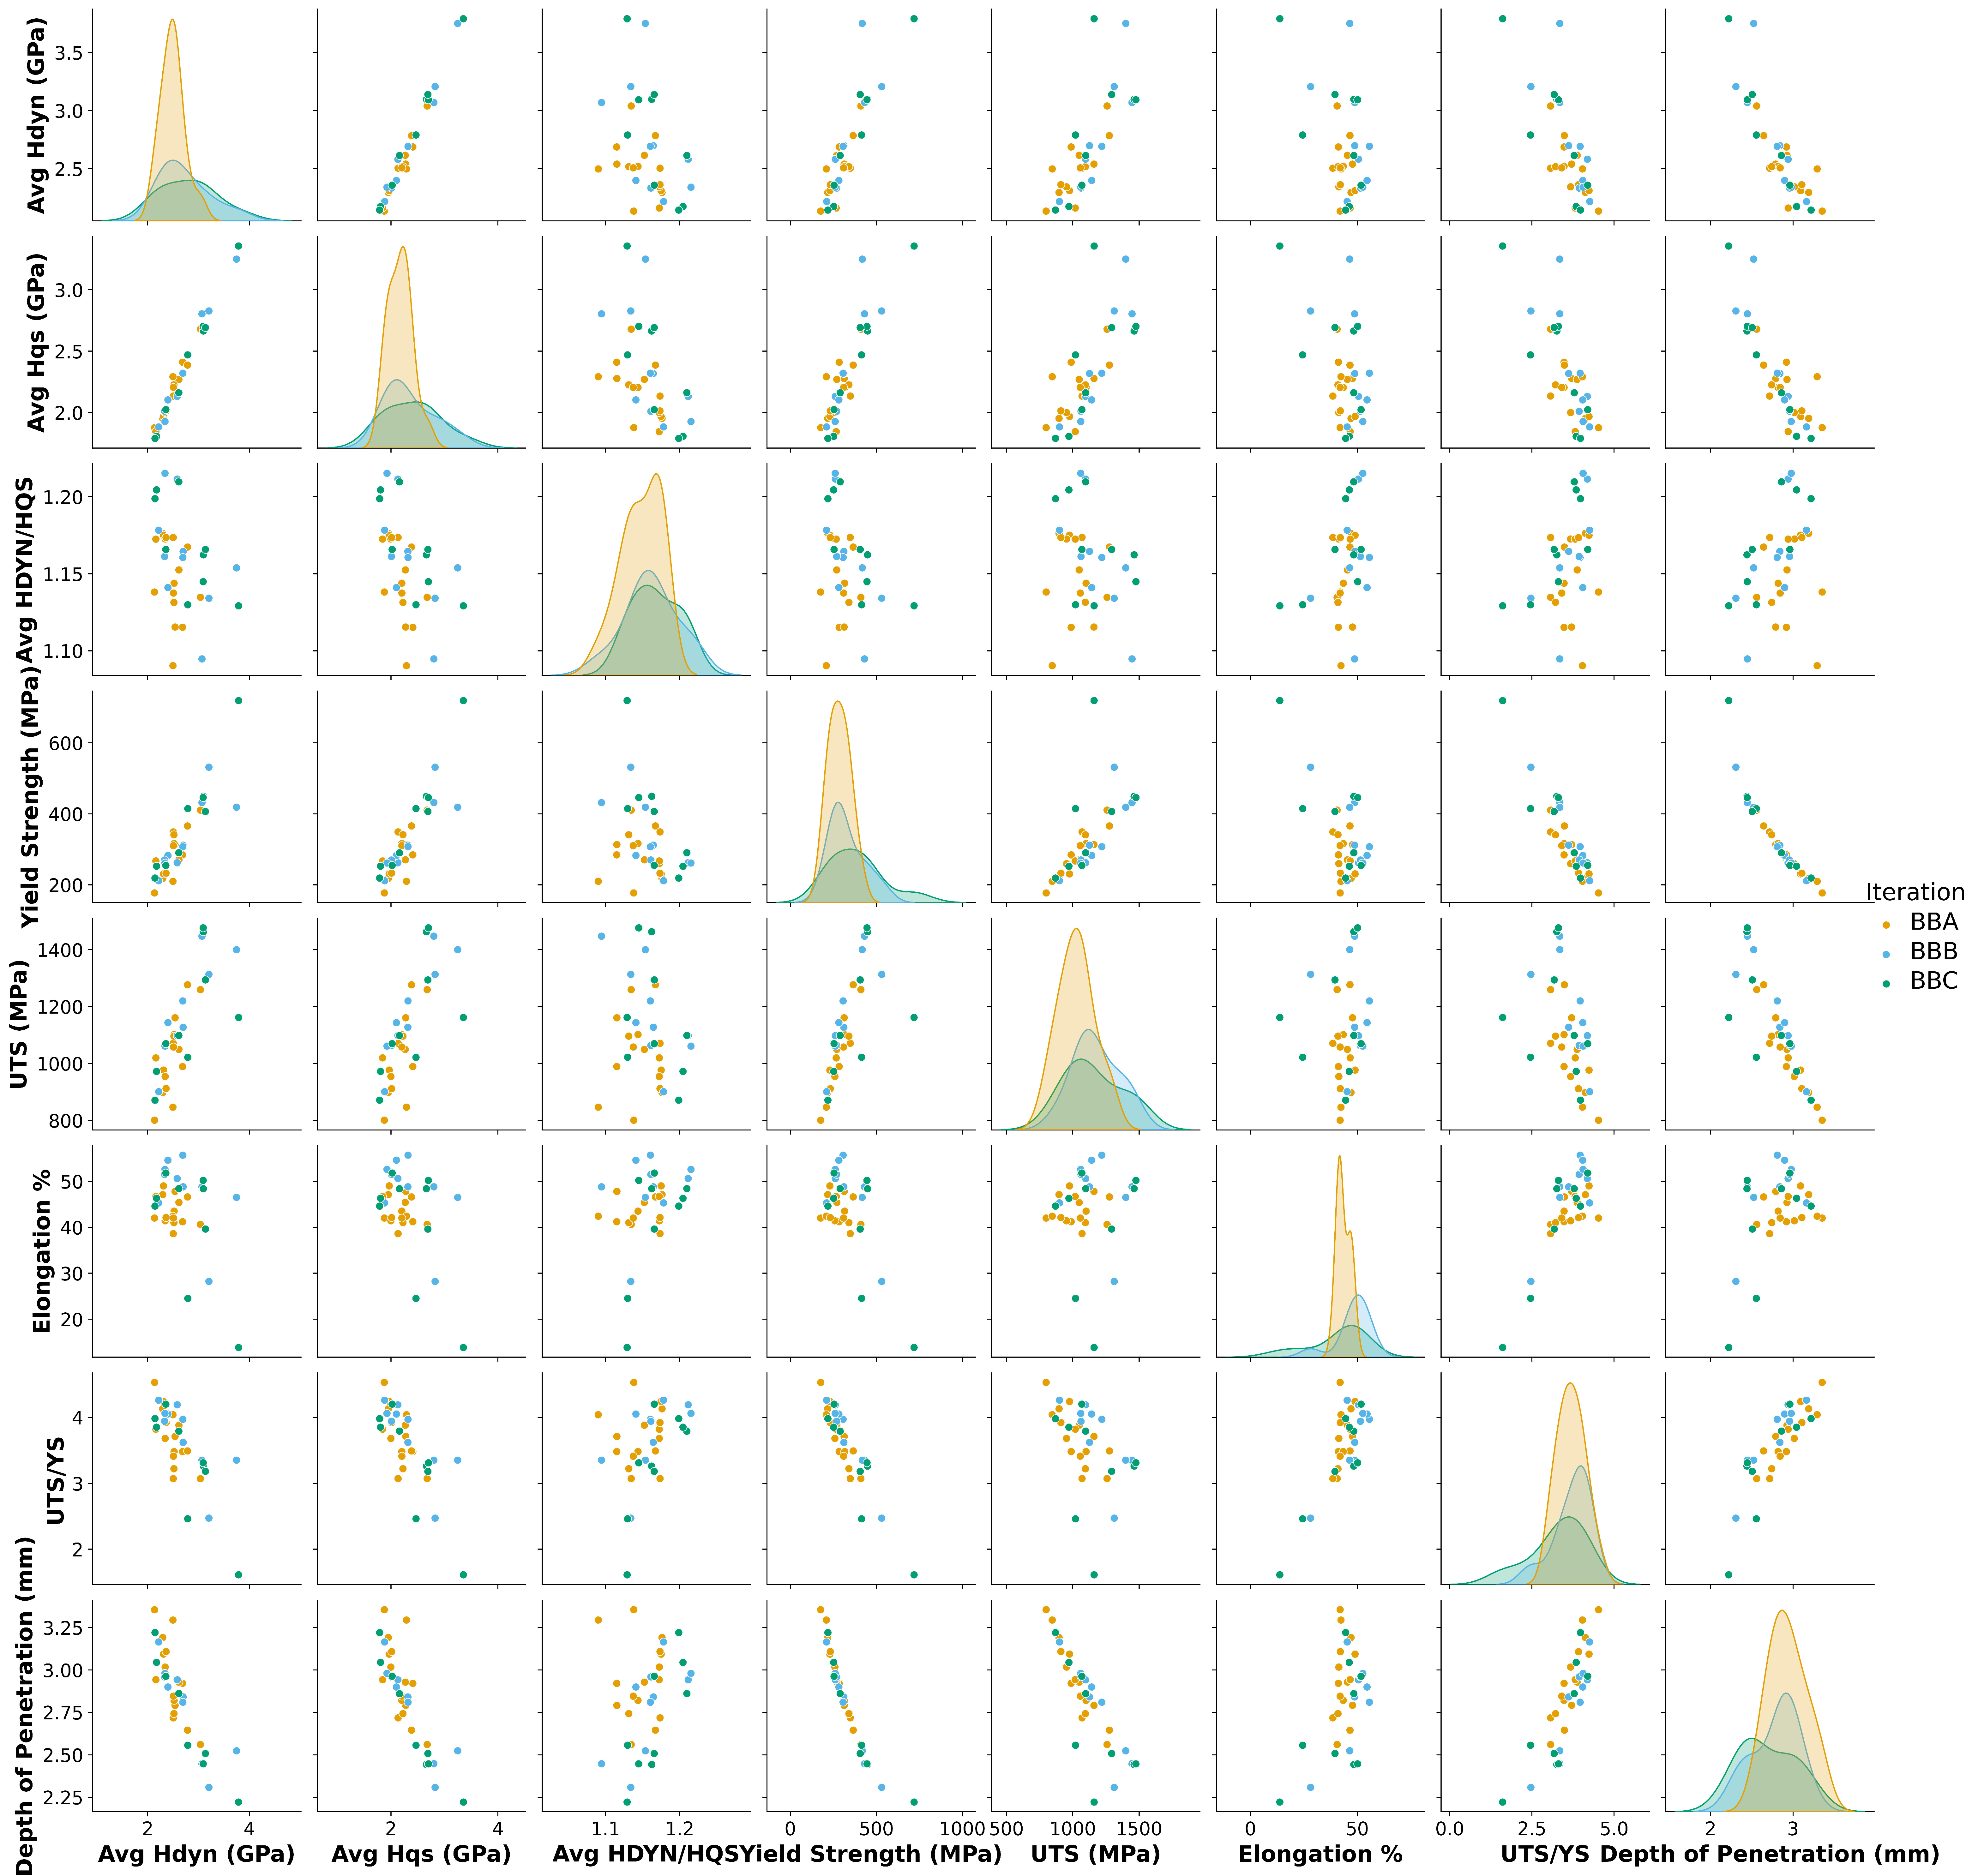
\includegraphics[width=0.9\textwidth]{Sup_figures/fig_si_09_property_pairplot.pdf}
    \caption{Comprehensive pairwise analysis of mechanical and ballistic properties for HEAs across all iterations within the study. Data points are color-coded by iteration: BBA (orange), BBB (blue), and BBC (green)}
    \label{fig:pairplot_correlations}
\end{figure*}


% Strong positive correlations are observed between strength-related properties (YS, UTS, Hdyn, Hqs), indicating that the optimization framework successfully identified compositional regions where multiple strength metrics improve simultaneously. This finding is particularly significant as it demonstrates that the high entropy alloy system enables concurrent enhancement of seemingly independent mechanical properties, challenging traditional materials design paradigms that often assume trade-offs between different strength measures.

% The correlation between dynamic and quasi-static properties reveals important insights for strain rate sensitive applications. The positive correlation between Hdyn and Hqs suggests fundamental material hardness improvements, while the distribution of Hdyn/Hqs ratios indicates varying degrees of strain-rate sensitivity across the alloy compositions. Alloys with higher Hdyn/Hqs ratios represent compositions that are particularly well-suited for high strain-rate applications such as ballistic protection.

Strong positive correlations are observed among the quasi-static strength metrics: YS and hardness are tightly coupled (r = 0.88), and the two hardness measures are nearly identical (r = 0.99). The strength–ductility trade-off characteristic of FCC HEAs is reflected in the UTS/YS ratio, which is strongly anticorrelated with YS (r = -0.91) and positively correlated with elongation (r = 0.80).

Depth of penetration shows a near-perfect inverse correlation with YS (r = -0.94) and a strong inverse correlation with UTS (r = -0.86), indicating that penetration resistance in this alloy family is governed predominantly by quasi-static strength. The four highest-YS single-phase FCC alloys identified by the campaign (BBC04, BBC02, BBB01, BBB12) are accordingly also the best simulated ballistic performers.

The Hdyn/Hqs ratio quantifies rate-dependent strengthening at the indentation scale. Across the campaign it spans a narrow range (1.09–1.22) with no clear single-element compositional trend. At the per-alloy level, the rate-dependent component of ballistic response is captured more directly by the calibrated Cowper–Symonds exponent M, which correlates positively with DoP and negatively with YS. The highest-strength alloys show lower rate-sensitivity exponents, a trade-off that is invisible to quasi-static testing alone. The Hdyn/Hqs ratio is therefore retained as a complementary rate-sensitive objective within the Bayesian optimization loop rather than as a stand-alone predictor of ballistic performance.






\clearpage
\setstretch{1.0}
% bibliographystyle already set in preamble
\bibliography{references}
\end{document}
